\chapter{DEMO: Mobile Manipulation in Human-shared Retail Spaces}
\label{cha:rss_24}

%% The following annotation is customary for chapter which have already been
%% published as a paper.
\blfootnote{
  \copysubmittedcontentfootnote
  \begin{itemize}
    \item \rssdemo
  \end{itemize}
  \statementcontributions{M. Spahn, C. Pezzato and C. Salmi were responsible for the
  software development and system integration. M. Spahn developed the trajectory
  generation method, C. Pezzato developed the reactive decision making method, and
  R. Dekker developed the perception system. The digital twin was implemented by
  C. Wang. C. Pek, J. Kober, J. Alonso-Mora, C. Hernandez Corbato, and M. Wisse
  positioned the work in the context of retail environments and provided
  infrastructure and guidance in all implemantation phases. M. Spahn led the
  writing process. All authors contributed to the final manuscript.}
}

%% It is only necessary to list the authors if multiple people contributed
%% significantly to the chapter.

\added{
\begin{abstract}
In the previous chapter, we have defined \ac{tg} as the problem of finding a
sequence of actions that will move the robot from its current state to a
desired state. As this thesis focuses on \ac{tg} for mobile manipulation,
relevant literature must therefore include works from different fields, ranging
from autonomous driving and mobile robotics to manipulation. Besides, \ac{tg} in
dynamic environments generally includes path planning and local \ac{tg}.
Therefore, this chapter summarizes approaches ordered on a scale of reactivity,
that is the frequency at which trajectories are computed. Starting with
controller-like \ac{tg} methods, we then move in order of increasing
time-horizon up until global path planning.
\end{abstract}

}

\newpage

%%%%%%%%%%%%%%%%%%%%%%%%%%%%%%%%%%%%%%%%%%%%%%%%%%%%%%%%%%%%%%%%%%%%%%%%%%%%%%%%

\section{Introduction}
\label{sec:introduction}

%\MW{We need still an appealing and convincing introduction. I think this is the best part for you to write. While doing this, you might want to look at the following section and remove all the repetitions in there.}


Ageing has started to impact the labour markets profoundly, and robotic labour shortage relief is becoming a necessity in all industries~\cite{mcgrath2021report,astrov2021economies}. Yet, there are still surprisingly few robots operating outside of structured environments. To bring robots successfully to human-occupied environments, the main challenge still is handling human-instilled disturbances~\cite{rodriguez2021human}, e.g., misplaced products in shelves, newly added products, blocked aisles, or interactions from humans. Such disturbances should be handled adaptively, with little development effort and short response times for natural effective interaction. 
Focusing on these challenges, this paper demonstrates a combination of two novel methods, one for adaptive decision making and one for rapid motion planning, embedded in a state-of-the-art integrated robot system. 

The demonstrator is a mobile manipulator for order picking in realistic supermarkets, see \cref{fig:layouts}. %In the following, we explain how this demonstrator is rooted in a real need. 
The increase in online shopping  induces an equal decrease in store visits. Especially in dense urban areas, these costly but conveniently located stores could have a dual use as distribution centres for flash delivery of online orders \cite{kronmuller2023online}. This requires the order picking to occur during opening hours, amongst store customers. We have taken this as our demonstrator scenario, but the methods are generally applicable for any scenario involving human-disturbed mobile manipulation tasks. In such scenarios, we assume that humans can block the robot's path, physically push or hold the manipulator, and move the pick-able items, before, during, or after a pick. Even if items are taken away from the robot's suction gripper, it should recover by picking another item of the same product. % of the same kind.
%

\begin{figure}
  \centering
  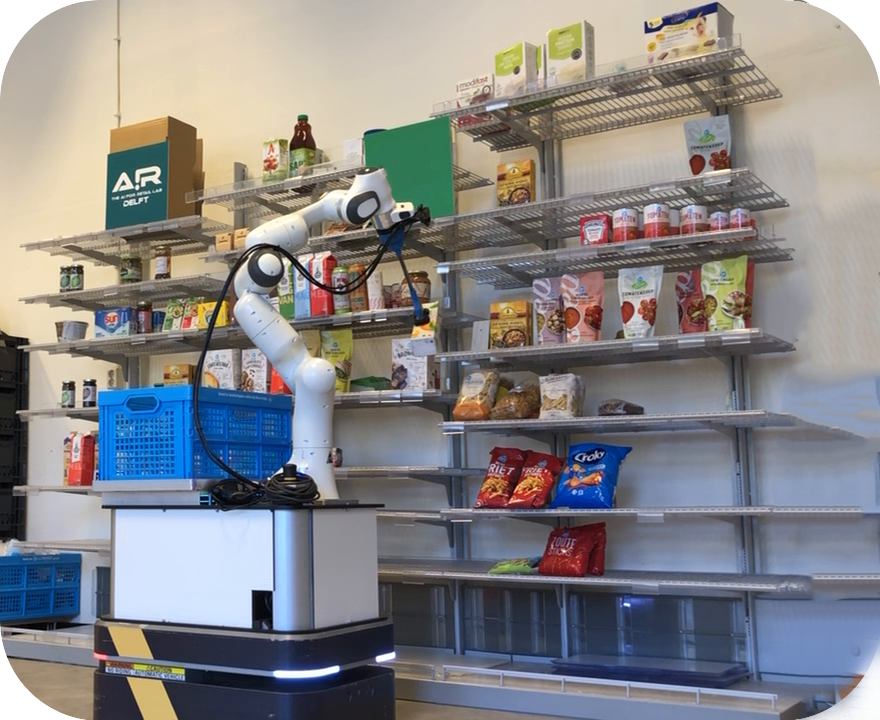
\includegraphics[height=140pt]{layout_lab_wo.png}
  \caption{We validated our mobile manipulator in our AIRLab lab environment (shown here) and a realistic supermarket environment of a large Dutch retailer. %Robot Hardware used for in the demo in the two evaluated environments. 
  %The robot is
  %composed out of a differential-drive robotic base and a
  %7-dof robotic arm.}
  }
  \label{fig:layouts}
\end{figure}
%Past demo papers at RSS, \cite{li2023large,deepmind2023demonstrating,toyota2023}

%Although the realization of such an %application is deemed simple
% To deploy autonomous robots in supermarkets with success, their operation in a
% human-shared environment must be safe, 
% fault-tolerant, and adaptive.
This work presents our mobile manipulation solution
in human-shared environments that aims at being adaptive and fault-tolerant. %Doing so, 
We focus on three main questions that are most 
relevant when deploying robots in supermarkets: How can we

\begin{enumerate}
  \item generate \emph{safe} and \emph{robust} trajectories for manipulation? % (safety, robustness)? %be robust, safe and easy to adapt by
  %non-experts (ease-of-use)?
  \item ensure \emph{fault-tolerant} task planning and execution? % (fault-tolerance)? 
  \item easily \emph{adapt} the robot to pick new products? % (adaptability)?
  %data-driven item detection be extended quickly (extendability)?
\end{enumerate}
Our solution addresses these questions with specific decisions on the robot's capabilities for decision-making, trajectory generation, and perception. Our contributions are thus an integrated system with adaptive decision-making, fast motion planning and easy-to-use teaching from demonstration. 

\section{Related Works}%
\label{sec:related_works}

Past works devoted to motion planning for mobile manipulators can be divided
into two main categories: optimization-based and sampling-based methods
\cite{LaValle2006,Mukadam2017}. Sampling-based methods, such as rapidly
exploring random trees (RRT's) \cite{Webb2013,Kleinbort2019,Kuffner2000} and
probabilistic roadmaps (PRM's) \cite{Hsu2002,Faust2017} are highly efficient at
generating paths for systems with high-degree of freedom. However, these
approaches consider static environments requiring a complete replanning if the
conditions change and hence, are not applicable for dynamic environments
\cite{Avanzini2018}.

In contrast, trajectory planning methods focus on executing generated paths
while avoiding collisions in dynamic environments. collisions developing motion
planning methods for mobile manipulators, most approaches either tackle the
motion planning problem for the robot's base or the robot's arm. Pioneer works
on motion planning methods for statically mounted manipulators employed
potential fields for collision avoidance \cite{Khatib1985}. Building on the
previous, \cite{Haddadin2011} introduced the Circular Field method to address
dynamic collision avoidance. Finally, to ensure collision avoidance for the
end-effector when grasping a moving obstacle, \cite{Du2018} employed a
repulsive vector.

\subsection{Collision Avoidance For Mobile Robots}
The dynamic window approach \cite{Fox1997} and its new variant proposed in
\cite{Zhang2019} have proven to be efficient in generating smooth trajectories
for mobile robots in static and dynamic environments. To navigate among
pedestrians, \cite{Ferrer2013} introduced the Social Forces model imitating
the human navigation behavior and using it as navigation policy for the
robot..  Yet, Social Forces and its variants rely on handcrafted functions
limiting their ability to handle more complex navigation scenarios. To deal
with a large number of agents, \textit{ORCA} was proposed in
\cite{VanDenBerg2011} and later extended for non-holonomic bases in
\cite{Alonso-Mora2012a}. However, these approaches demonstrate highly reactive
behaviors because they only consider one step look-ahead predictions. MPC
schemes were proposed for mobile robots and autonomous vehicles in
\cite{Brito2019} and \cite{Schwarting2018} allowing to optimize over a
prediction horizon and avoid, in advance, dynamic obstacles. To enable coupled
control of a mobile manipulator, collision avoidance must be performed in the
3D space which is usually not necessary for ground vehicles. Several 3D MPC
formulation were proposed for drones to enable safe motion through cluttered
environments \cite{Tordesillas2019,Liu2017}.

\subsection{Collision Avoidance For Mobile Manipulators}
Despite abundant research in trajectory planning for mobile robots and robotic
arms, few works focused on coupling both systems' control. It was shown that
coupling the base and the robotic arm motion leads to a considerable reduction
of total operational time and smoother motions \cite{Thakar2018, Thakar2019}.
Nevertheless, these methods were designed for static environments and did not
allow real-time collision avoidance. Furthermore, trajectory planning for the
coupled system is a precondition for effective interactive navigation, including
opening doors \cite{Jain2009, Chitta2010} or moving obstacles out of the way
\cite{Li2019}.

In the context of mobile manipulation, less research focused on collision
avoidance in dynamic environments, including changing scenes and moving
obstacles. A real-time controller using MPC was presented in \cite{Ide2011}, in
which either a holonomic or a non-holonomic base was combined with a
two-degree-of-freedom robotic arm mounted onto the base. Although hardware
constraints were respected, no collision avoidance was considered.  An MPC
formulation for mobile manipulators with holonomic bases that allows collision
avoidance was presented in \cite{Avanzini2015}. The perceived obstacles were
translated into a set of spheres to be respected by the MPC scheme. The proposed
approach used dynamically changing weights to change between arm motion and
locomotion, resulting in a locked arm during navigation. A different weight
setting was used to perform motion underneath a horizontal bar with an a priori
position. The work is extended to non-holonomic bases and includes object
detection in moving underneath the horizontal bar \cite{Avanzini2018}. 

\section{System overview}

We briefly introduce the considered supermarket setting and
detail our order picking pipeline and system components.

\subsection{Considered supermarket setting}

Modern supermarkets are characterized by a large range of
products, around 100,000 different products per store.
Operators usually have access to detailed information of all
those products, including mass, geometry, and shelf location
in the store. In our demonstration, we assume that the robot
can access this database to inform its decision. The large
variety of products usually requires specialized grasping
strategies per category, e.g., grasping tomatoes is
different from grasping a large soft\hyp{}drink bottle. We focus
on a subset of products that can be picked with the suction
gripper of our robot (see hardware design in
\cref{sec:hardware}), e.g., cans, milk boxes, bottles, or
bags of crisps (see \cref{fig:product_examples}). The masses
of products range from 100g (instant food mixes) to 1.5 kg
(soft\hyp{}drink bottle) and the size are between 10 cm (cans)
and 30 cm (soft\hyp{}drink bottle). We assume that products to
pick are visible, accessible from the shelf's front and in the robot's workspace.
\begin{figure}[t]
  \centering
  \begin{subfigure}[b]{0.20\linewidth}
    \centering
    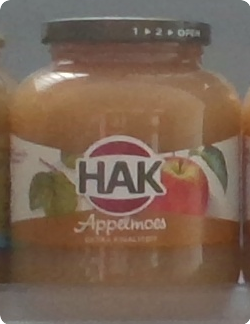
\includegraphics[height=1.2\textwidth]{appelmoes_rounded.png}
  \end{subfigure}%
  \begin{subfigure}[b]{0.20\linewidth}
    \centering
    
\includegraphics[height=1.2\textwidth]{fries_rounded.png}
  \end{subfigure}%
  \begin{subfigure}[b]{0.20\linewidth}
    \centering
    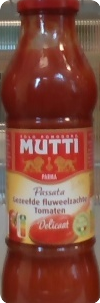
\includegraphics[height=1.2\textwidth]{mutti_rounded.png}
  \end{subfigure}%
  \begin{subfigure}[b]{0.20\linewidth}
    \centering
    
\includegraphics[height=1.2\textwidth]{soup_rounded.png}
  \end{subfigure}%
  \caption{Examples of different products considered in this
  work.}
  \label{fig:product_examples}
\end{figure}

%Moreover, in the interest of bridging the gap between robotics research and applications on the market, achieving high reliability for a part of all products is assumed to be favorable. Besides, 
For in\hyp{}store picking, we focus on picking products
during opening\hyp{}hours and favor reliability over execution speed. 
%, because warehouse automation is already being tackled by redesigning the interior making collaborative robots obsolete
%in such environments. Based on this focus, we generally favor reliability over execution speed. 

\subsection{Hardware}
\label{sec:hardware}

Our mobile manipulator platform is comprised of various hardware components. 

\paragraph{Robot}
The mobile manipulator is composed of two robots, see
\cref{fig:hardware}. The moving base is a Clearpath Boxer,
differential drive wheeled-robot that can achieve similar
speeds to humans while having a relatively small footprint.
The robotic arm is a
Franka Emika Panda, a serial manipulator with seven degrees
of freedom, equipped with torque sensors in every joint that
can achieve high accuarcy while being safe to work around,
see \cref{fig:layouts}. The attached gripper is a custom
3D-printed suction gripper with two suction cups powered by
a industrial vacuum pump.
\begin{figure}[t]
    \centering
    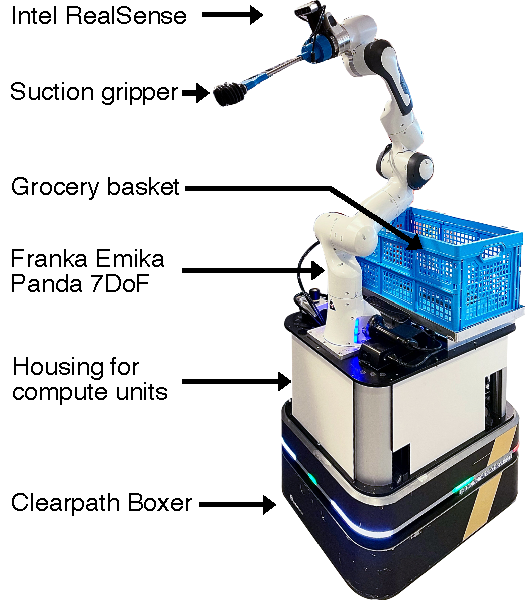
\includegraphics[width=0.65\linewidth]{AlbertHWIntro.pdf}
    \caption{Overview of our robot's hardware.}
    \label{fig:hardware}
\end{figure}


\paragraph{Perception}
The base uses a 270 degree Lidar sensor to localize itself
and detect dynamic obstacles and humans in the environment.
We mounted a Realsense D435 RGBD camera on the wrist link of
the arm and use it to detect products and perform visual
servoing during picking.

\paragraph{Compute Units}
We use a total of four compute units to distribute the computational load of individual software components. 
The first compute unit is the Franka Control Interface controlling the arm. 
The base's compute unit performs
self-localization and collision avoidance for the base.
The central compute
unit is an Intel NUC with an Intel i7 10th generation CPU, running all planning components and the user interface for placing orders. 
%Object detection and localization is
%running on an separate laptop mounted on the top of the robot, below the shopping
A Dell Alienware laptop mounted on the robot with an RTX 3070 TI GPU runs the perception components. %perform
%inference on the detector network and image processing.
Our two computers are running the Robot Operating System (ROS) and communicate via a network switch.


\subsection{Order\hyp{}picking overview}
\label{sec:order_system_overview}



\begin{figure*}[ht]
  \centering
  \begin{subfigure}[b]{0.18\linewidth}
    \centering
    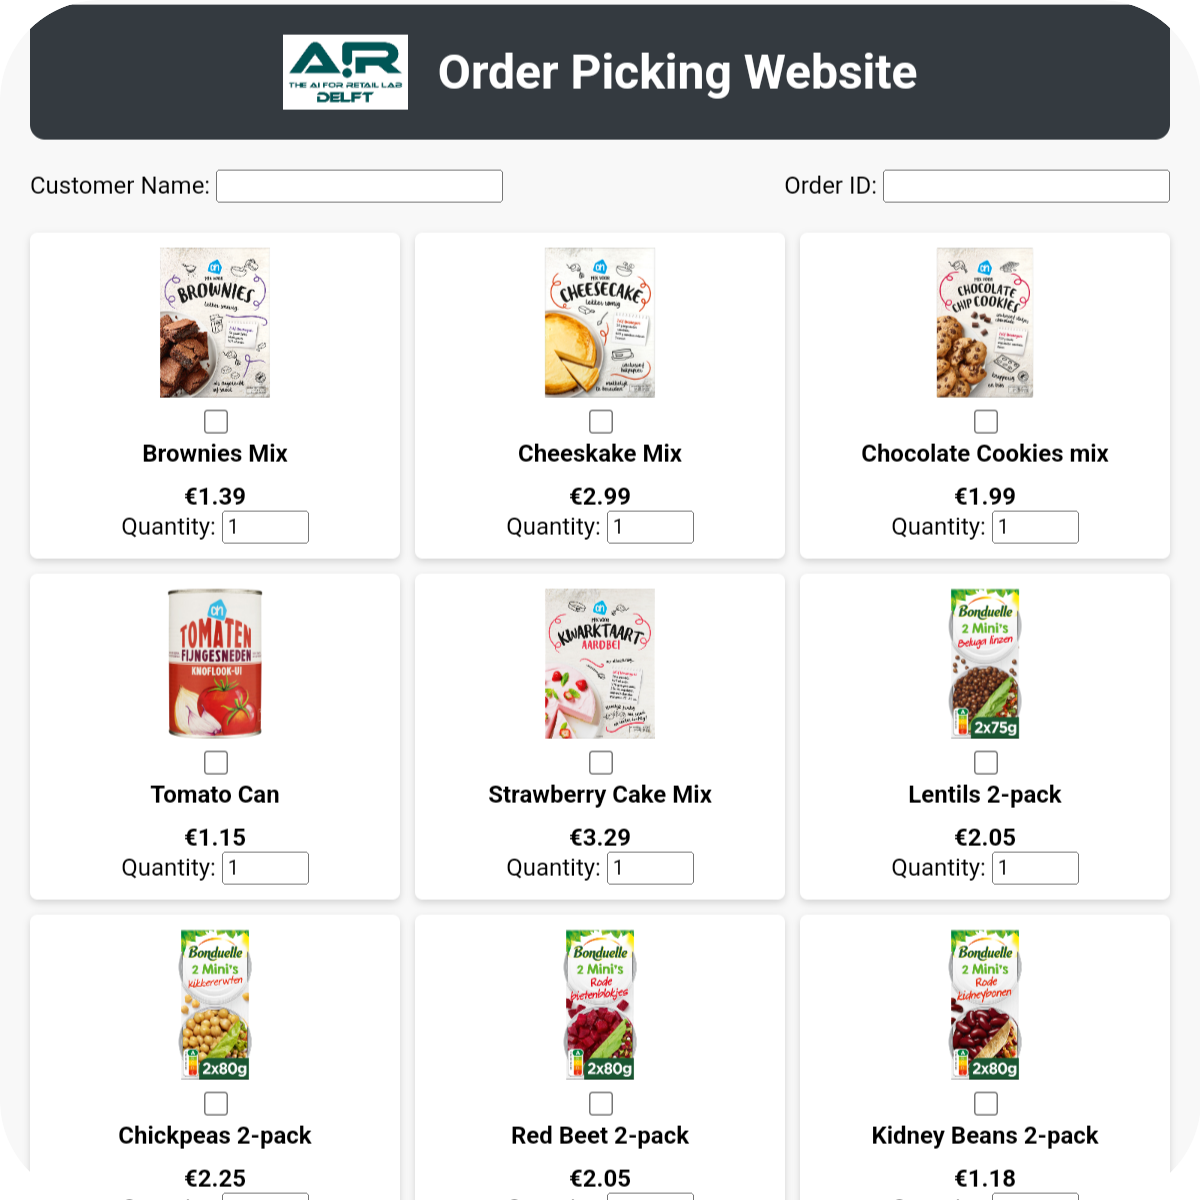
\includegraphics[width=1\textwidth]{order_interface.png}
    \caption{Customer order}
  \end{subfigure}%
  \begin{subfigure}[b]{0.18\linewidth}
    \centering
    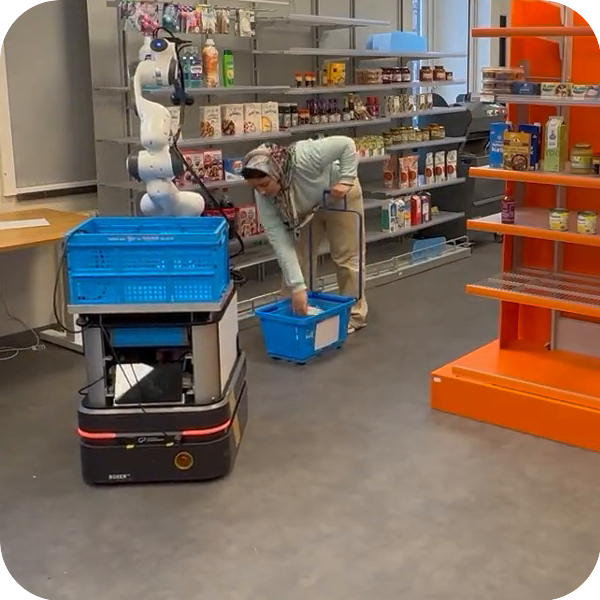
\includegraphics[width=1\textwidth]{navigation.png}
    \caption{Navigate to shelf}
  \end{subfigure}
  \begin{subfigure}[b]{0.18\linewidth}
    \centering
    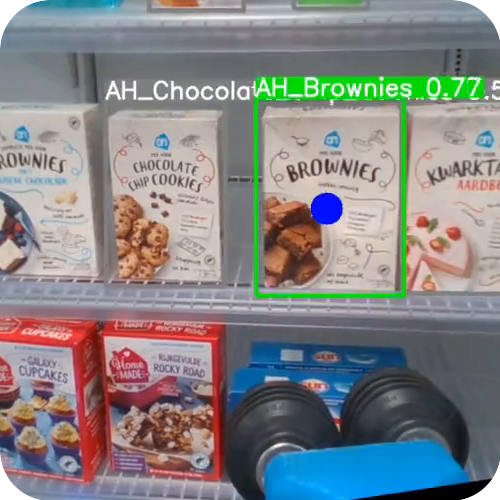
\includegraphics[width=1\textwidth]{locate_item.png}
    \caption{Locate item}
  \end{subfigure}
  \begin{subfigure}[b]{0.18\linewidth}
    \centering
    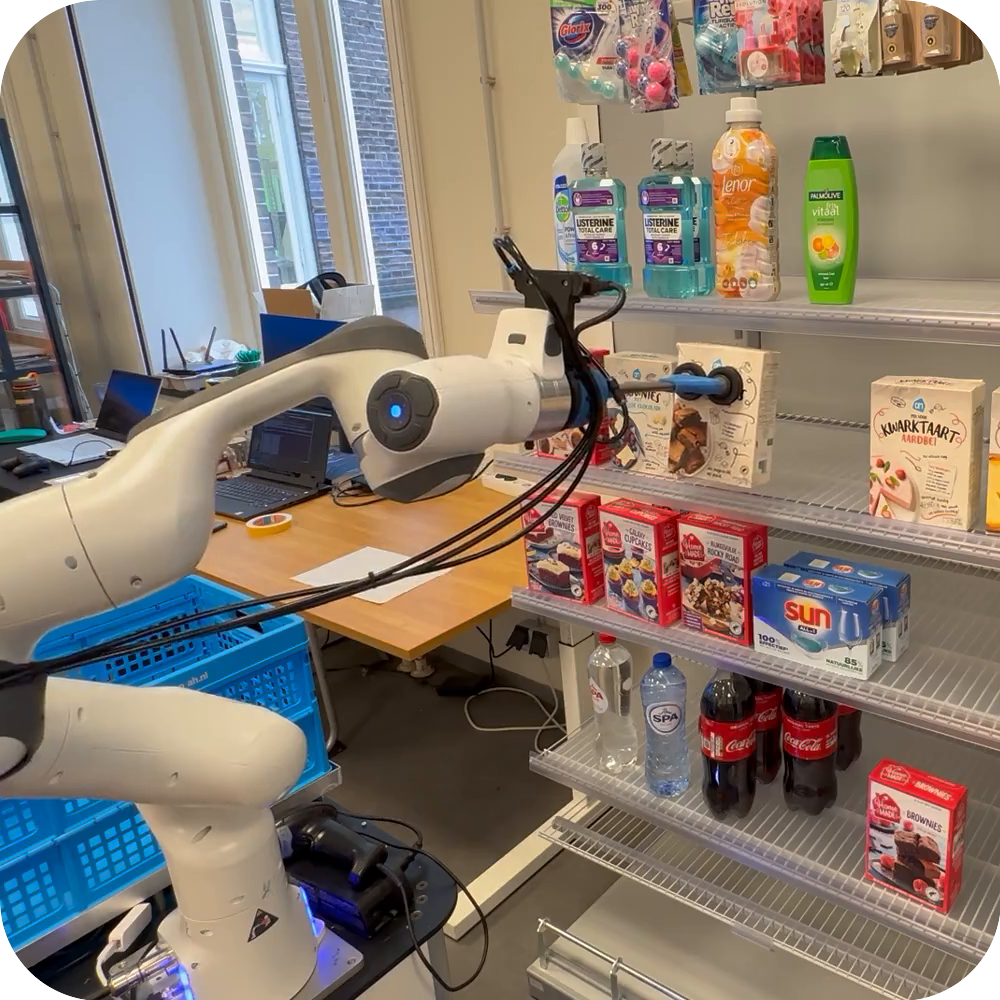
\includegraphics[width=1\textwidth]{picking.png}
    \caption{Pick item}
  \end{subfigure}
  \begin{subfigure}[b]{0.18\linewidth}
    \centering
    \includegraphics[width=1\textwidth]{placing.png}
    \caption{Place item}
  \end{subfigure}
  \caption{Overview of ideal flow of symbolic actions to complete an order.}
  \label{fig:flow}
\end{figure*}


%A static sequence of tasks for order-picking in supermarkets can roughly be described as follows.
%
The high\hyp{}level overview of our order\hyp{}picking system is
illustrated in \cref{fig:flow}.
Customers first place an order via the order placement website. 
The robot processes the order into a task assignment. 
For each item, it navigates to the item's shelf, locates it, picks and places it in the basket.
When the order is completed, the customer can pick up the order from the robot.





\subsection{System components}

We used the order\hyp{}picking sequence in \cref{sec:order_system_overview} to guide our system development, while focusing on adaptiveness to recover from failure and inaccuracies in perception. 
In the following, we outline the main
system components that are visualized in \cref{fig:software_overview} and can be grouped in: 
\begin{figure}[t]
  \begin{center}
    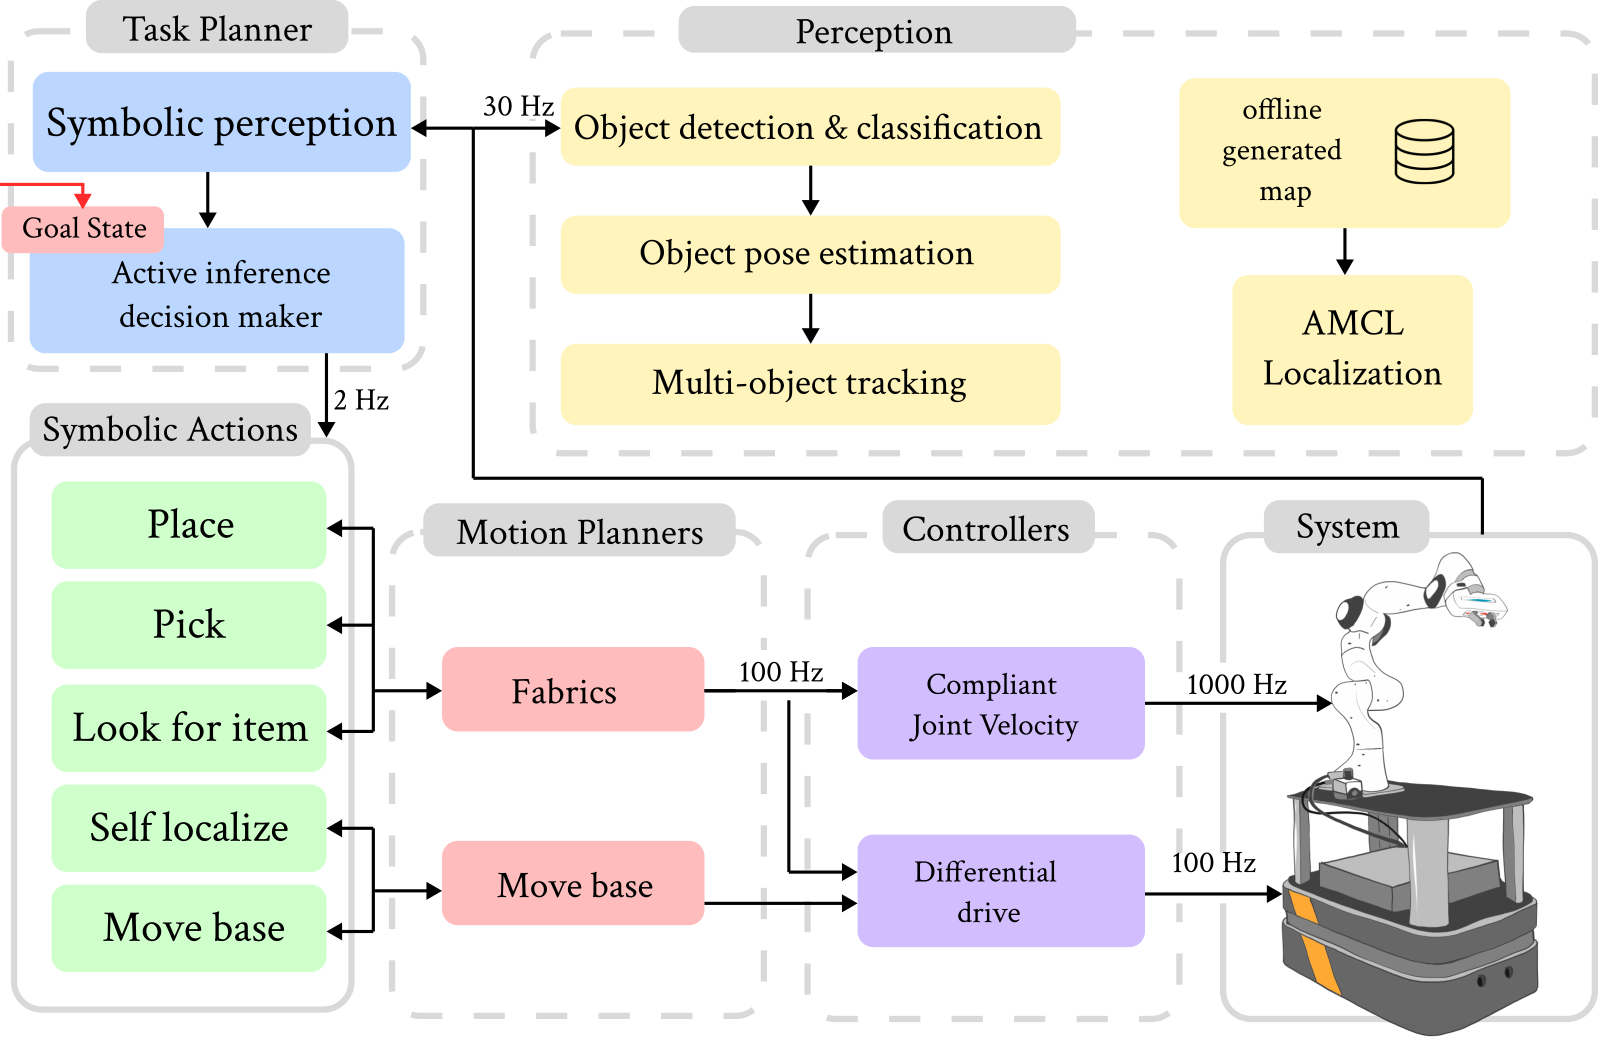
\includegraphics[width=1.00\linewidth]{overview_updated.png}
  \end{center}
  \caption{Overview of system components.}
  \label{fig:software_overview}
\end{figure}
%The overview of our system components is visualized in. 
(a) task planner, (b) motion planners, (c) low\hyp{}level controllers, and (d) perception.


After receiving the customer order, the task planner (see
\cref{sec:decision_making}) determines the order of picking
products by minimizing the robot's travelled distance. The
task planner uses a combination of a behavior tree and
symbolic state information, such as the robot is holding a
product or has arrived at the desired position,
with an adaptive inference method to determine the best next
symbolic action to execute.
We define a \textit{symbolic action} as an elementary robot
behavior. Symbolic actions can be as simple as greeting the
customer or as complex as picking an item.
We use a set of five robot
symbolic actions:
picking items, placing items, looking for items, localizing
the robot, and navigating the robot. Each symbolic action is realized
by the motion planning and control components (see
\cref{sec:trajectory_generation}). Motion planning is
decomposed into path planning and online trajectory
optimization for the base and reactive trajectory generation
for the arm, augmented with a pseudo\hyp{}prismatic joint on the
base, see \cref{sec:trajectory_generation}. Lastly, the
perception component (see \cref{sec:perception}) takes care
of item detection and classification and provides item poses
to the planning components.

\section{Task Planning and Execution}
\label{sec:decision_making}

Once the customer submits an order, the Task Planner creates
a plan to collect the items in the order throughout the store and bring the shopping basket to the delivery location.

Our decision-making approach to creating these plans and executing them is designed explicitly with failure recovery in mind. It consists of i) offline plans that leverage the known structure of the task, and ii) online planning to adapt the sequence of actions to unforeseen disturbances, following the approach in \cite{pezzato2023active}. Offline planning involves planning a sequence of desired states as leaf nodes in a behavior tree --- instead of the standard action nodes--- to send task sub-goals to the online active inference planner. The latter is an online planner that computes an action sequence to transition from the current state to the next desired one.

\subsubsection{Offline planning}

The structure of the task is modelled offline as a plan to be executed using the template behavior tree shown in Fig.~\ref{fig:bt_full} and expanded by Fig.~\ref{fig:subtree}, making the robot try to pick every product up to $N$ times, and then deliver the groceries to the delivery location.
It specifies an initial welcome to the customer, a ``Product Subtree'' slot, an active inference node that sets the final task sub-goal of being at the delivery location for the online active inference planner, and a closing message to the customer.  For each product, a sub-tree as in Fig.~\ref{fig:subtree} is created automatically. Following the ordered list, every sub-tree for each product is inserted in the overall BT structure from Fig.~\ref{fig:bt_full}, as part of the sequence.
%The overall BT will  


\begin{figure}[b!]
    \centering
    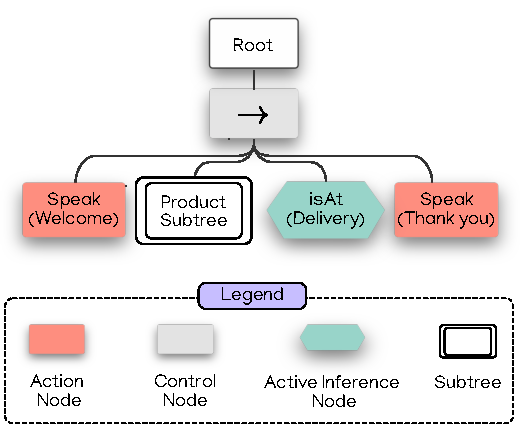
\includegraphics[width=0.8\linewidth]{bt_full.pdf}
    \caption{Overall Behavior Tree structure. The action \texttt{Speak{}} interfaces with the voice module to produce a suitable message for the customers (see Sec.~\ref{sec:teaching}).}
    \label{fig:bt_full}
\end{figure}



\begin{figure}[b!]
    \centering
    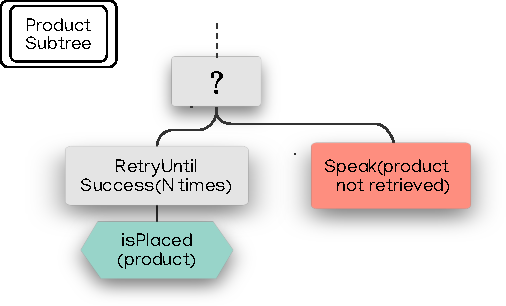
\includegraphics[width=0.8\linewidth]{bt_subtree.pdf}
    \caption{Sub-tree structure for placing an item in the basket. The active inference node sets a prior over the state \texttt{isPlaced{}} for a product, triggering the online decision-making. The action \texttt{Speak{}} produces a voice message to explain the failure in case one happens (see Sec.~\ref{sec:teaching}).}
    \label{fig:subtree}
\end{figure}




\subsubsection{Online planning with Active Inference} 

The active inference planner (AIP) takes the task sub-goals \texttt{isPlaced} and \texttt{isAt} as desired states of items being placed in the robot's basket and the robot being at the delivery location respectively, and computes a plan of symbolic actions based on the robot's skills that achieves those states.
Our planner is based on discrete active inference, which relies on a generative model that contains beliefs about future states and action plans, where plans that lead to preferred states are more likely. The preferred action sequence is the one with the highest probability of achieving desired states. 

Our active inference planner rests on the tuple $(\mathcal{O},\mathcal{S},\mathcal{A})$. This is composed of a finite set of observations $\mathcal{O}$, a finite set of symbolic states $\mathcal{S}$, and a finite set of symbolic actions $\mathcal{A}$ that correspond to the robot's skills.


The continuous state of the world $x\in\mathcal{X}$ is discretized through a symbolic observer into boolean variables about the relevant states of the world, e.g., item held by the gripper. These discrete observations $o$ are used to build a probabilistic belief about the symbolic current state, described in Table~\ref{tab:States}.



The AIP computes the posterior distribution over $p$ plans $\bm \pi$ through free-energy minimization \cite{pezzato2023active}. The symbolic action to be executed by a robot in the next time step is the first action of the most likely plan, denoted with $\pi_{\zeta, 0}$:
\begin{eqnarray}
\label{eq:a_t}
    \zeta = \max(\underbrace{[\bm\pi_{1}, \bm\pi_{2},...,\bm\pi_{p}]}_{\bm \pi^\top}),\ 
    a_{\tau=0} = \pi_{\zeta, 0}.
\end{eqnarray}




\begin{table}[ht!]
\caption{Notation for states}% title of Table
\centering % used for centering table
%\begin{tabular}{C{2.8cm} C{4.7cm}} % 
\begin{tabular}{c c} % 
\toprule %inserts double horizontal lines
\textbf{State, Boolean State} & \textbf{Description}\\ [0.5ex] % 
\midrule % inserts single horizontal line
${s^{(at)}},\ {l^{(at)}}$ & Belief about being at the goal location \\
${s^{(loc)}},\ {l^{(loc)}}$ & Belief about being self-localized \\
${s^{(reach)}},\ {l^{(reach)}}$ & Belief about reachability of an object\\
${s^{(hold)}},\ {l^{(hold)}}$ & Belief about holding an object\\
${s^{(vis)}},\ {l^{(vis)}}$ & Belief about an object being in sight\\
${s^{(place)}},\ {l^{(place)}}$ & Belief about an object being placed at a location\\
\midrule
\textbf{Boolean State} & \textbf{Common Name}\\ [0.5ex] % 
\midrule % inserts single horizontal line
${l^{(at)}= [1\ 0]^\top}$ & \texttt{isAt(goal\slash obj)} \\
${l^{(loc)}= [1\ 0]^\top}$ & \texttt{isLocalized} \\
${l^{(reach)}= [1\ 0]^\top}$ & \texttt{isReachable(obj)}\\
${l^{(hold)}= [1\ 0]^\top}$ & \texttt{isHolding(obj)}\\
${l^{(vis)}= [1\ 0]^\top}$ & \texttt{isVisible(obj)}\\
${l^{(place)}= [1\ 0]^\top}$ & \texttt{isPlaced(obj)}\\
\bottomrule %inserts single line
\end{tabular}
\label{tab:States}
\end{table}

% \begin{table}[ht!]
% \caption{Common name for states}% title of Table
% \centering % used for centering table
% \begin{tabular}{C{3cm} C{3cm}} % 
% \toprule %inserts double horizontal lines
% \textbf{Boolean State} & \textbf{Common Name}\\ [0.5ex] % 
% \midrule % inserts single horizontal line
% ${l^{(at)}= [1\ 0]^\top}$ & \texttt{isAt(goal\slash obj)} \\
% ${l^{(loc)}= [1\ 0]^\top}$ & \texttt{isLocalized} \\
% ${l^{(reach)}= [1\ 0]^\top}$ & \texttt{isReachable(obj)}\\
% ${l^{(hold)}= [1\ 0]^\top}$ & \texttt{isHolding(obj)}\\
% ${l^{(vis)}= [1\ 0]^\top}$ & \texttt{isVisible(obj)}\\
% ${l^{(place)}= [1\ 0]^\top}$ & \texttt{isPlaced(obj)}\\
% \bottomrule %inserts single line
% \end{tabular}
% \label{tab:common_names}
% \end{table}

\begin{table}[h]
\caption{Notation for actions}% title of Table
\centering % used for centering table
\begin{tabular}{p{2.5cm}p{2.5cm}p{2.5cm}} % centered columns (4 columns)
\toprule
    \textbf{Actions}& \textbf{Preconditions}& \textbf{Postconditions}\\ 
    \midrule
    \texttt{selfLoc()} & \texttt{-} & \texttt{isLocalized} \\
    \texttt{moveTo(goal\slash obj)} & \texttt{isLocalized} & \texttt{isAt(goal)}\slash \\
    & & \texttt{isReachable(obj)} \\  
    \texttt{pick(obj)} & \texttt{isReachable(obj)}& \texttt{isHolding(obj)}\\ 
     & \texttt{!isHolding} & \\
     & \texttt{isVisible(obj)} & \\
    \texttt{place(obj)} & \texttt{isHolding}& \texttt{isPlaced(obj)}\\
    &  & \texttt{!isHolding(obj)}\\
    \texttt{look(obj)} & \texttt{-} & \texttt{isVisible(obj)}\\
    \bottomrule
\end{tabular}
\end{table}
%
%\CP{postconditions naming and isAt etc should match}
%

The combination of offline plans modelled as behaviour trees and online planning using active inference facilitates responsive action selection for long-term tasks within partially observable and dynamic environments, which is particularly crucial in addressing disturbances in retail settings. 

 This approach offers the advantage of not having to account for every conceivable contingency and recovery behavior within a Behavior Tree, and at the same time allows for continuous online planning.
 This effectively minimizes computational complexity, enabling the development of a robot capable of adhering to predefined routines while also adapting locally to unforeseen events through real-time online planning with active inference.

\section{Trajectory generation}
\label{sec:trajectory_generation}


In the following, we detail the various approaches we employ for real time trajectory generation (Sec.~\ref{sub:base_motion}, \ref{sub:arm_motion}). Furthermore, we highlight the look for product (Sec.~\ref{sub:look_for_product}), pick (Sec.~\ref{sub:picking}) and place (Sec.~\ref{sub:place}) skills introduced in Fig.~\ref{fig:software_overview} and we explain how they use the trajectory generation approaches. %Finally, we cover our teaching approach (\ref{sub:teaching}), inspired by learning-from-demonstration, that provides grasping trajectories to the picking skill.

\subsection{Navigation of the base}
\label{sub:base_motion}
To navigate the mobile base in the store we employ the MoveBase navigation framework, configured with A* as the global planner and Timed-Elastic-Bands as the local planner \cite{rosmann2017integrated}.
We record a map of the environment including static obstacles prior to deployment.
Additionally, we manually define a keep-out
area to prevent the robot from going into unsafe or crowded areas, such as the checkout zones. The local planner employs the environment map and online lidar sensor information for avoiding collisions with static and moving obstacles, such as humans.

\subsection{Motion of the arm}
\label{sub:arm_motion}
To generate the motion of the arm (and base during picking), we employ the framework of \ac{fabrics}.
Fabrics is based on the composition of behaviours, defined as differential equations in the appropriate manifolds, which enables safe real-time planning at a very high frequency \cite{ratliff2023fabrics,van2022geometric,spahn2023}. Since \ac{fabrics} is a local, reactive trajectory generation method, global guidance is required to perform complex actions, such as product picking or placing. 
The global guidance for fabrics essentially consists of a sequence of local goals, where we only continue to the next goal if the previous goal has been reached. In Sec.~\ref{sub:teaching} we show how this sequence of goals, i.e., reference trajectory, can be obtained by human teaching. In the following we shortly explain how \ac{fabrics} works and how to use it.



\subsubsection{Method}
Requirements such as collision avoidance, joint-limit avoidance or self-collision avoidance are referred to in fabrics as behavioral components. Each component is represented as a differential equation of the form
$\M(\x,\xdot)\xddot+\f(\x,\xdot)=\nullvec$ on an appropriate
manifold \X{} of the configuration space \Q{}, where \M{} and \f{} are the importance metric and the forcing term respectively, and $\x$, $\xdot$ and $\xddot$ are the state, e.g., full configuration of the robot or end effector pose, and its derivatives in the manifold \X{}.
By respecting
simple construction rules, each behavioral component can be ensured to
be an optimization fabric, i.e., a dynamic system that is
stable by construction. All components can then be combined
in the robot's configuration space by applying the
operations of \textit{pull-back} and \textit{summation}. In
the configuration space, we obtain one optimization fabrics
of the form $\M\qddot + \f = \nullvec$, where $\qddot$ is the second derivative of the configuration and $\M$ and $\f$ the resulting importance metric and forcing term, respectively.
We define goal states of the robotic arm as a set of
constraints $\Sc = \{\Con_1,\Con_i,\Con_n\}$ where each
constraint \Con{} is defined by the tuple
$\Con=(\fk{p},\fk{c},\x)$. Here, $\fk{p}$ is the forward
kinematics to the parent link, $\fk{c}$ the forward
kinematics to the child link, and $\x$ is the desired position
vector. These constraints are implemented in \ac{fabrics} as a forcing term with the
differential map $\map_{\textrm{goal}} = (\fk{c} - \fk{p}) -
\x$. On the manifold defined by this differential map, we
define the forcing potential $\forc$ that can be pulled at
forcing our optimization fabric as
$\M\qddot+\f+\der{\q}{\forc} = 0$.
For further details on the definition and composition of fabrics we refer the reader to \cite{spahn2023}.

The key advantages of \ac{fabrics} are their very fast computation and their flexibility to
compose behaviours and define the desired goal in an appropriate manifold, rather than being
fixed to defining a target configuration or end-effector pose. For
example, some tasks may require to align the end-effector
to face a point in the workspace, while
the actual position along the line is of little importance,
\cref{fig:look_for_product}.
To give another example, some products, like a can, can be grasped from many directions and one may only need to specify a subset of the desired grasping pose, e.g., the height at which the can is grasped and that the grasp should be perpendicular to the vertical axis, but not the specific direction of approach.


\begin{figure}[b]
  \centering
  \begin{subfigure}[b]{0.5\linewidth}
    \centering
    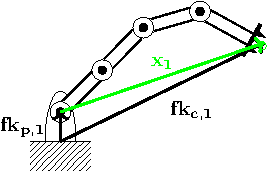
\includegraphics[width=1\textwidth]{one_constraint.pdf}
    \caption{}
    \label{subfig:one_goal_constraint}
  \end{subfigure}%
  \begin{subfigure}[b]{0.5\linewidth}
    \centering
    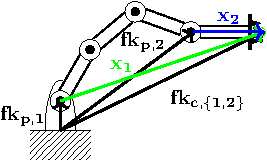
\includegraphics[width=1\textwidth]{two_constraints.pdf}
    \caption{}
    \label{subfig:two_goal_constraints}
  \end{subfigure}
  \caption{Goal constraints for \ac{fabrics}. In (a), 
  the only constraint is defined by $\Con_1 = (\fk{p,1},
  \fk{c,1}, \x_1)$.
  In (b), a second constraint is added as
   $\Con_2 = (\fk{p,2}, \fk{c,2}, \x_2)$ to align the
   end-effector horizontally.}
  \label{fig:goal_constraints}
\end{figure}

\subsubsection{Usage} As an example, a reaching problem, where the
end-effector should be at a certain position is defined by
$\Con_{\textrm{ee}} = (\fk{0},\fk{ee},\x_\textrm{ee})$,
where $\fk{0}$ is the forward kinematics to the base link of
the robot and $\x_\textrm{ee}$ the desired position of the
end-effector in the base link frame. See \cref{fig:goal_constraints} for two examples of composing goal states by constraints.

A problem we encountered when picking products with only the arm, is that the workspace of the arm is limited w.r.t. the size of the shelf. This in combination with variability in base position or product location, often resulted in the product being out of reach or requiring difficult arm configurations close to joint limits.
%As the workspace of the arm is quite limited, base navigation can be quite inaccurate, and product locations might be disturbed by other customers,
Therefore, during the picking skill, we augment arm motion by integrating the forward motion of the base as a pseudo-prismatic joint to the kinematic chain. This can be easily done in \ac{fabrics} by appending the base motion to the state vectors \q{}, \qdot{}, and \qddot{}, see \cref{fig:base_motion}. 


\subsection{Look for a product}
\label{sub:look_for_product}
Looking for the product is triggered as soon as the robotic
base is placed in front of the shelf that is expected to
have the desired product. The camera frame is then located
at a position $\x_{\camera}$. Now, the camera
must be pointed towards the expected product location, defined as
$\x_{\product}$. We can model this goal as two
constraints. First, the camera link should not move from its
current location, thus $\Con_1 =
(\fk{0},\fk{camera},\x_{\textrm{camera}})$. Secondly, the
camera should face the product location. We can compute the
ray connecting the camera and the product location
$\x_{\textrm{ray}} = \x_{\product} - \x_{\camera}$ to then
define $\Con_2 = (\fk{7}, \fk{8},  \x_{\textrm{ray}})$
that effectively aligns the end-effector with the previously
defined ray $\x_{\textrm{ray}}$, see
\cref{fig:look_for_product}.

\begin{figure}
  \begin{center}
    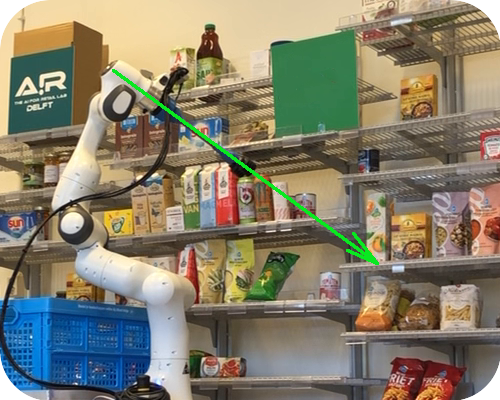
\includegraphics[width=0.55\linewidth]{look_for_item_wo.png}
  \end{center}
  \caption{Illustration of the orientation constraints for trajectory
  generation for the look-for-product skill.}
  \label{fig:look_for_product}
\end{figure}


\subsection{Picking of a product}
\label{sub:picking}
To define a goal for picking products we use a combination of three constraints.
First, the position of the vacuum cup is determined by the
position of the product, thus $\Con_1 =
(\fk{0},\fk{suction-cup}, \x_{\textrm{suction}}, \weight_{\textrm{suction}})$. Secondly, we
limit  ourselves to picking products from the shelf, thus
constraining the end-effector to be perpendicular to the
shelf by defining $\Con_2 = (\fk{7},\fk{8}, \x_{7,8})$. Lastly, our gripper is composed of two
suction cups, which, depending on the product should align with a specific angle for executing the most reliable grasp. The desired alignment defines
our third constraint for the picking as $\Con_3 =
(\fk{suction1}, \fk{suction2}, \x_{\textrm{alignment}})$. Although it is possible to
program a picking action, including approach and retreat, as a sequence of this set of
constraints, it is difficult to capture all the nuances of
picking in the code. Therefore, we make use of a human operator to teach the robot the best trajectory to reliably pick specific products, following the 
learning-from-demonstration paradigm
\cite{celemin2022interactive}. Teaching has proven an effective way to generate sequences of the previously mentioned
constraints thus encoding the human understanding of the picking problem into recorded trajectories. We explain the process of
recording and playing back trajectories in detail in Sec.~\ref{sub:teaching}. 
%

%

\subsection{Placing of a product}
\label{sub:place}

Placing the product consists of four phases. The robot navigates
to a configuration to its right or to its left depending on
whether it was a right-sided pick or a left-sided pick.
Then, it moves above the crate facing downwards. This is
defined by two constraints, $\Con_1 = (\fk{0},\fk{8},
\x_{0,8}, 1)$ and $\Con_2 = (\fk{7},\fk{8}, \x_{7,8})$.
The product is then placed by moving the arm downwards until an
external force, from touching the bottom of the crate
or an already placed product, is detected. That triggers the
release of the gripper and changes the goal to the homing
position ready for the next product.
% In
% case, the robot is commanded with a goal defined in the
% configuration space, we limit motion to the arm. All other
% goals are composed as a union of \textit{goal-constraints}.
% A goal-constraint is a defined by a desired distance vector
% between two links on the kinematic chain. 









\section{Perception}
\label{sec:perception}

The three perception components are
shown in \cref{fig:software_overview}.
\begin{itemize}
    \item \textbf{Object detection and classification:}
      Generates 2D object proposals and classifies them in a
      binary way based on a provided target class, resulting
      in the proposals being classified as either target
      class or not. 
      Object detection and classification are realized using
      two different models. Both models are fine-tuned on a 
      supermarket dataset, but do not require retraining to
      add new products, as we will explain in the following.
    \item \textbf{Object pose estimation:} Uses 2D object
      proposals in combination with a depth image to convert
      them to 3D. To estimate the orientation around the
      z-axis, we use a plane-fit of the pointcloud frustum.
      That first order approximation of the surface of the
      products front has proven to be a reliable approach,
      even for non-planar surfaces, see
      \cref{fig:product_examples}.
    \item \textbf{Multi-object tracking:} To track the
      objects over time, we use a set of Kalman Filters, one
      per object. The object proposals are assigned to
      Kalman Filter tracks using the Hungarian Algorithm
      \cite{hamuda2018improved,sahbani2016kalman}.
\end{itemize}

Because a supermarket has a large and often changing set of
products, the main requirement for our perception pipeline
is that it should be easily adaptable. This observation from
retail environments led us to the constraint on the
perception pipeline that it should not require retraining
when new products are added. Such a constraint can be
addressed using, so-called, \textit{few-shot} models.
In the
following, we describe the details of our object detection
and classification method.

The method utilizes YOLO for object detection, relying on
product details for object classification. Additionally, our
system allows adding products using a
single or few images.

This dynamic addition of new products is possible trough a
few-shot model we dub ProtoProductNet. This model is based
on ProtoNet \cite{protonet_2017}. ProtoNet matches query
images to target classes by their distance in feature space.
For each target class a prototype is constructed that is
essentially the mean of the features of a number of example
images of this class. By matching query images to target
prototypes, ProtoNet essentially learns to encode features
that classify similarity between query images and target
classes. Because this model picks random query- and target
classes from a dataset for every iteration, ProtoNet learns
a general feature extraction strategy that is invariant of the
actual class. This is important for adding new
products, as classifying new products is as easy as
providing the model with new target images.

The exact implementation of ProtoNet we use is based on P$>$M$>$F \cite{pmf_2022}. P$>$M$>$F shows that in few-shot learning pre-training (P) is more important than meta-training (M), which is in turn more important than fine-tuning (F). For the best results the authors of P$>$M$>$F suggest using ProtoNet with a Vision Transformer pre-trained with DINO \cite{dino_2021} as the feature extractor and meta-training it with a small learning rate.

However like most few-shot classification models, ProtoNet assumes that query images can only be one  target class. Not only would comparing a query image to all supermarket products increase inference time, attributing it to a likeliest product is unsafe. If our product detector misidentifies a human as a product, the classifier must correctly recognize that and not classify it as the most likely product.

ProtoProductNet makes exactly this possible. It uses a ViT pre-trained with DINO to extract image features, and predicts if those features are part of a target prototype based on their cosine distance. ProtoProductNet then passes this cosine distance through a linear layer combined with a sigmoid function to translate it to a confidence score. If query images have a confidence $<0.5$, they are considered not the target class. Using a sigmoid function however leads to a loss of relational information between classes. In contrast to ProtoNet, that predicts only the most likely target class among a set of target classes with a softmax function, a sigmoid predictor only uses the cosine distance per class to make predictions. As this mechanic is an important reason why ProtoNet works so well, ProtoProductNet will also be allowed to choose the likeliest from a number of prototypes. This means that next to a target prototype, a number of helper prototypes will be chosen. When classes are likelier to be a helper class then the target class, they are considered to be not the target class. As classes that are close together in feature space are harder to distinguish, it makes only sense to choose helper prototypes that are close to the target prototype.

% \begin{figure}[ht]
  % \begin{center}
    % 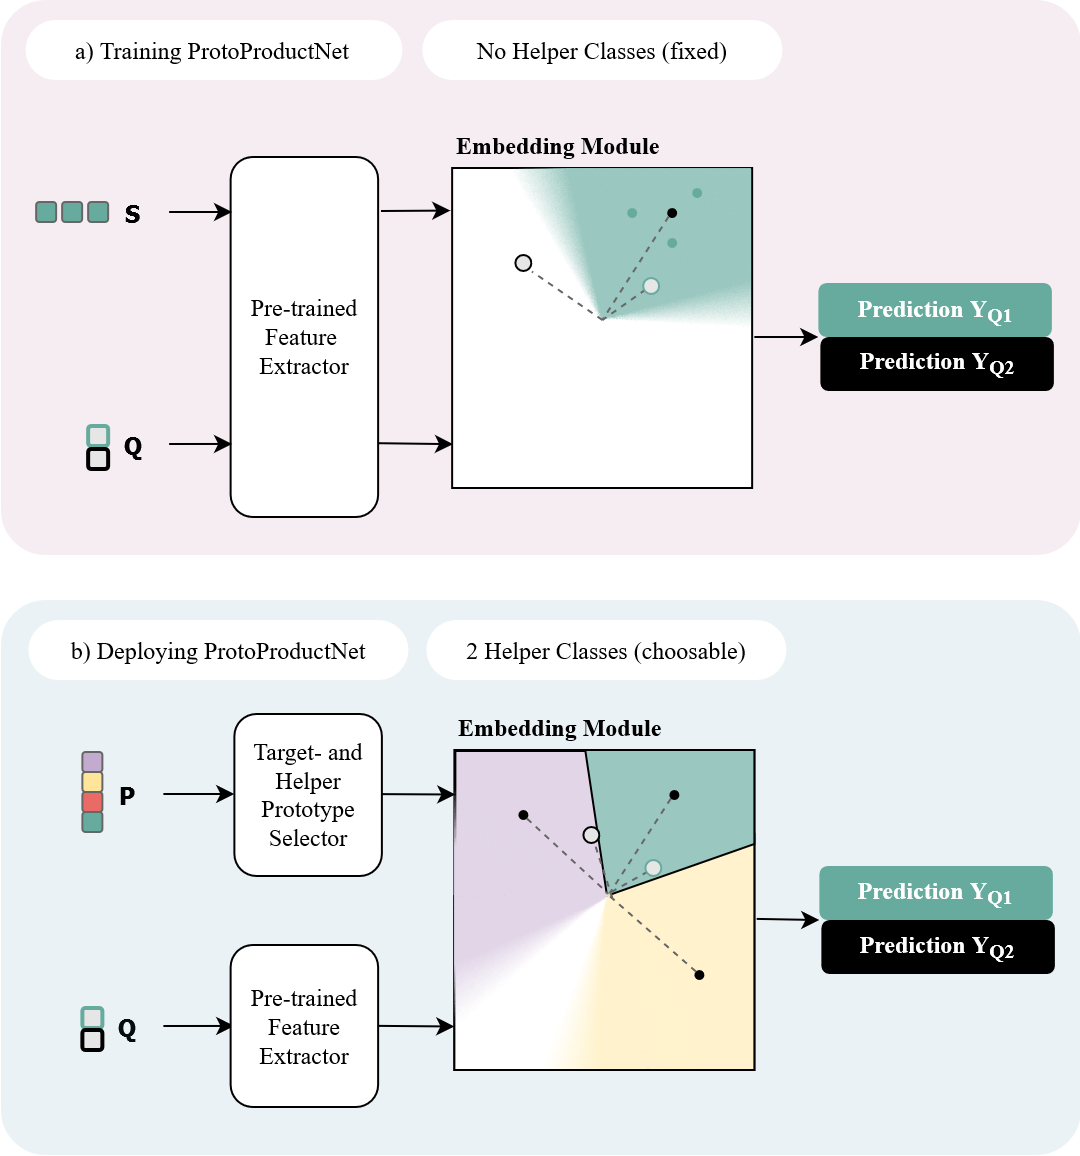
\includegraphics[width=0.95\linewidth]{rss_protoproductnet.png}
  % \end{center}
  % \caption{An overview of the architecture of ProtoProductNet during a) training; and b) deployment. Helper prototypes help distinguish close classes during inference.}
  % \label{fig:protoproductnet_overview}
% \end{figure}


\section{Interaction and Teaching Capabilities}
\label{sec:teaching}

To quickly adapt our robot to new store environments and
products, we created four interfaces for operators: a
digital twin for remote monitoring and control, adding
product classes to the perception, trajectory teaching mode,
and audio explanations of the robot's symbolic actions.

\subsection{Digital Twin for Remote Monitoring and Control}
\label{sec:digital_twin}

\begin{figure*}[t]
  \begin{center}
    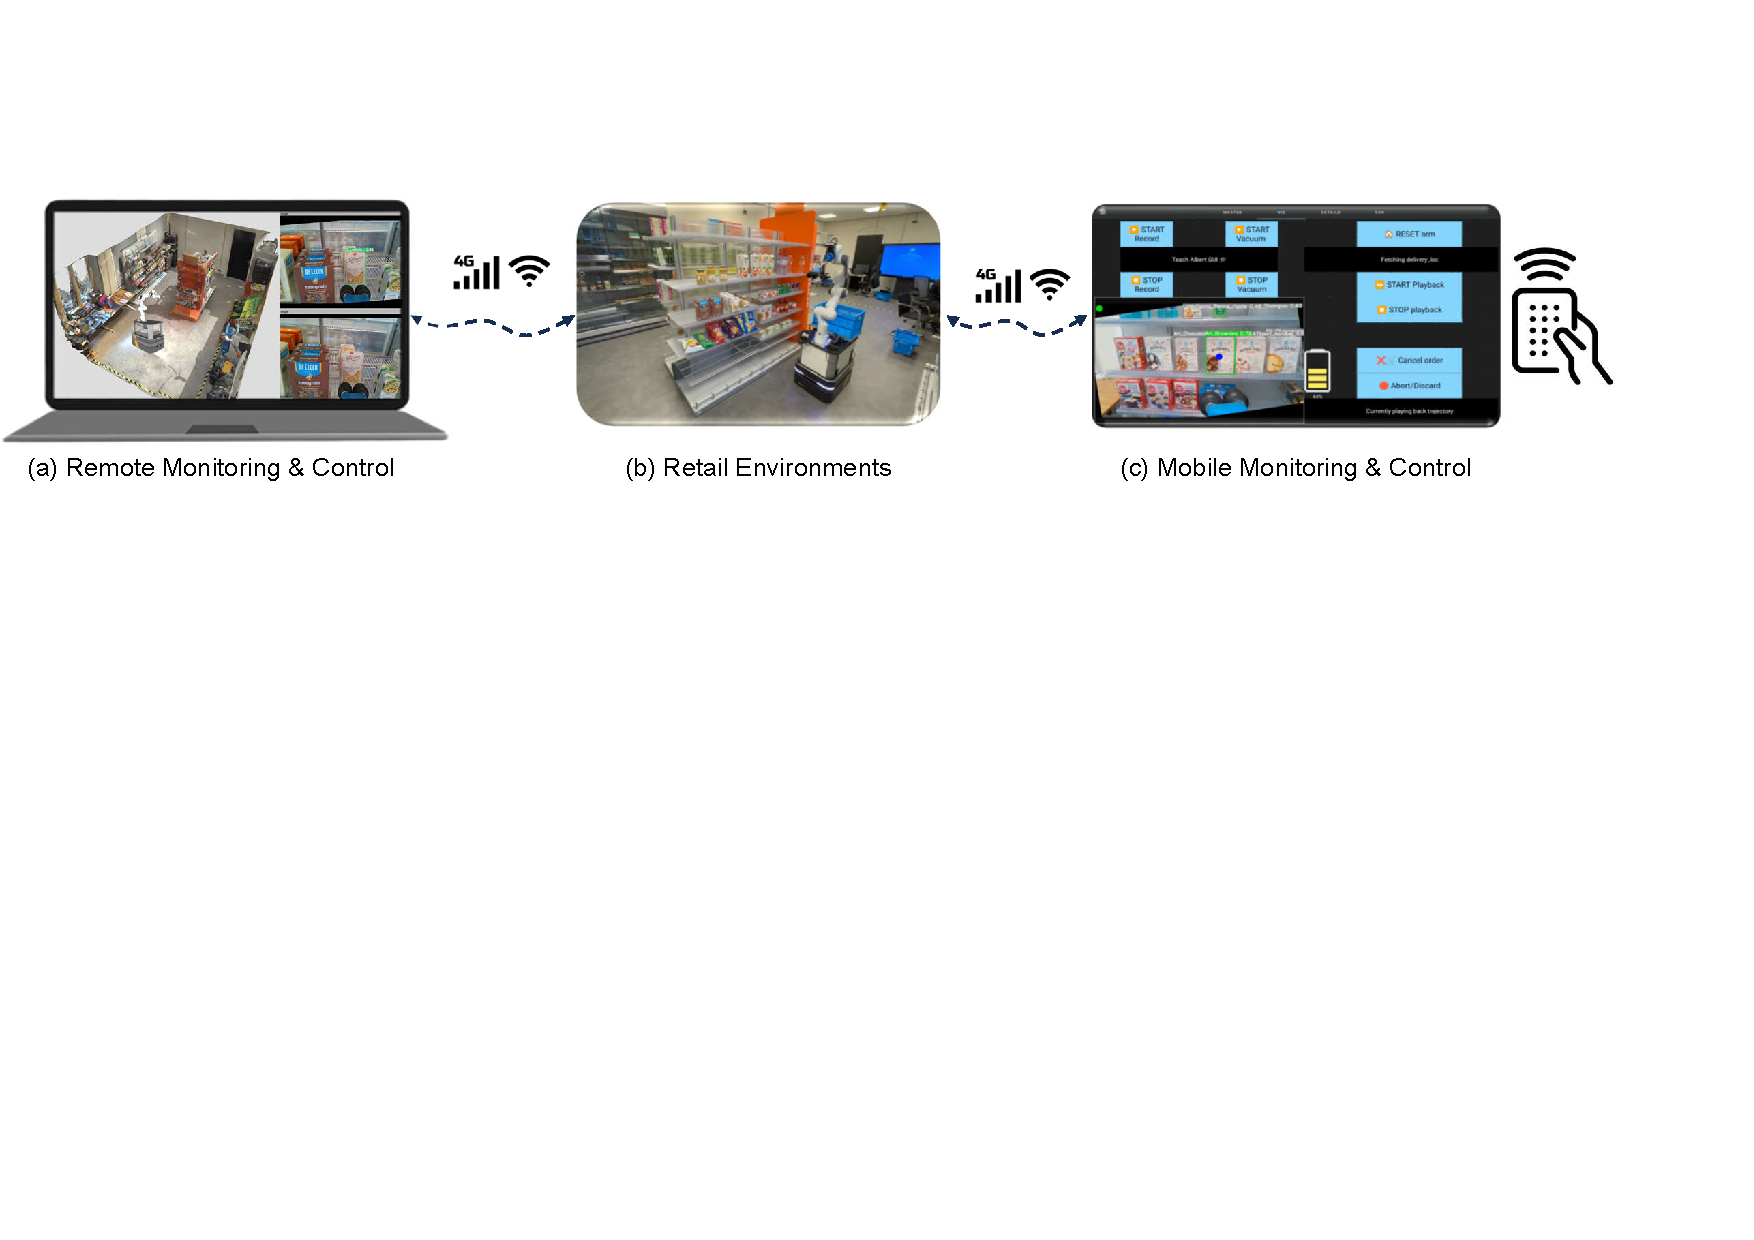
\includegraphics[width=0.85\linewidth]{remote_v5.pdf}
  \end{center}
  \caption{Overview of the remote monitoring and control system. a) Laptop-based remote interface for monitoring and control system; b) Visualization of the robot within the actual retail environment; c) Tablet interface for on-the-go monitoring and task programming}\label{fig:remote_overview}
\end{figure*}

Herein, we introduce a digital twin mechanism to support remote monitoring and control of a mobile manipulator in a retail setting, as shown in Fig.~\ref{fig:remote_overview}. By scanning the environment in three dimensions, we construct a virtual model that accurately represents the workspace. The robot, when operational in a supermarket, is connected to this digital twin through Wi-Fi or 4G, enabling operators to monitor its status and issue commands from any remote location. The addition of a tablet interface allows for flexible monitoring and control by on-site staff, who can easily adjust the robot's course or teach it new tasks as needed.




\begin{figure}[t]
  \centering
  \begin{subfigure}[b]{0.45\linewidth}
    \centering
    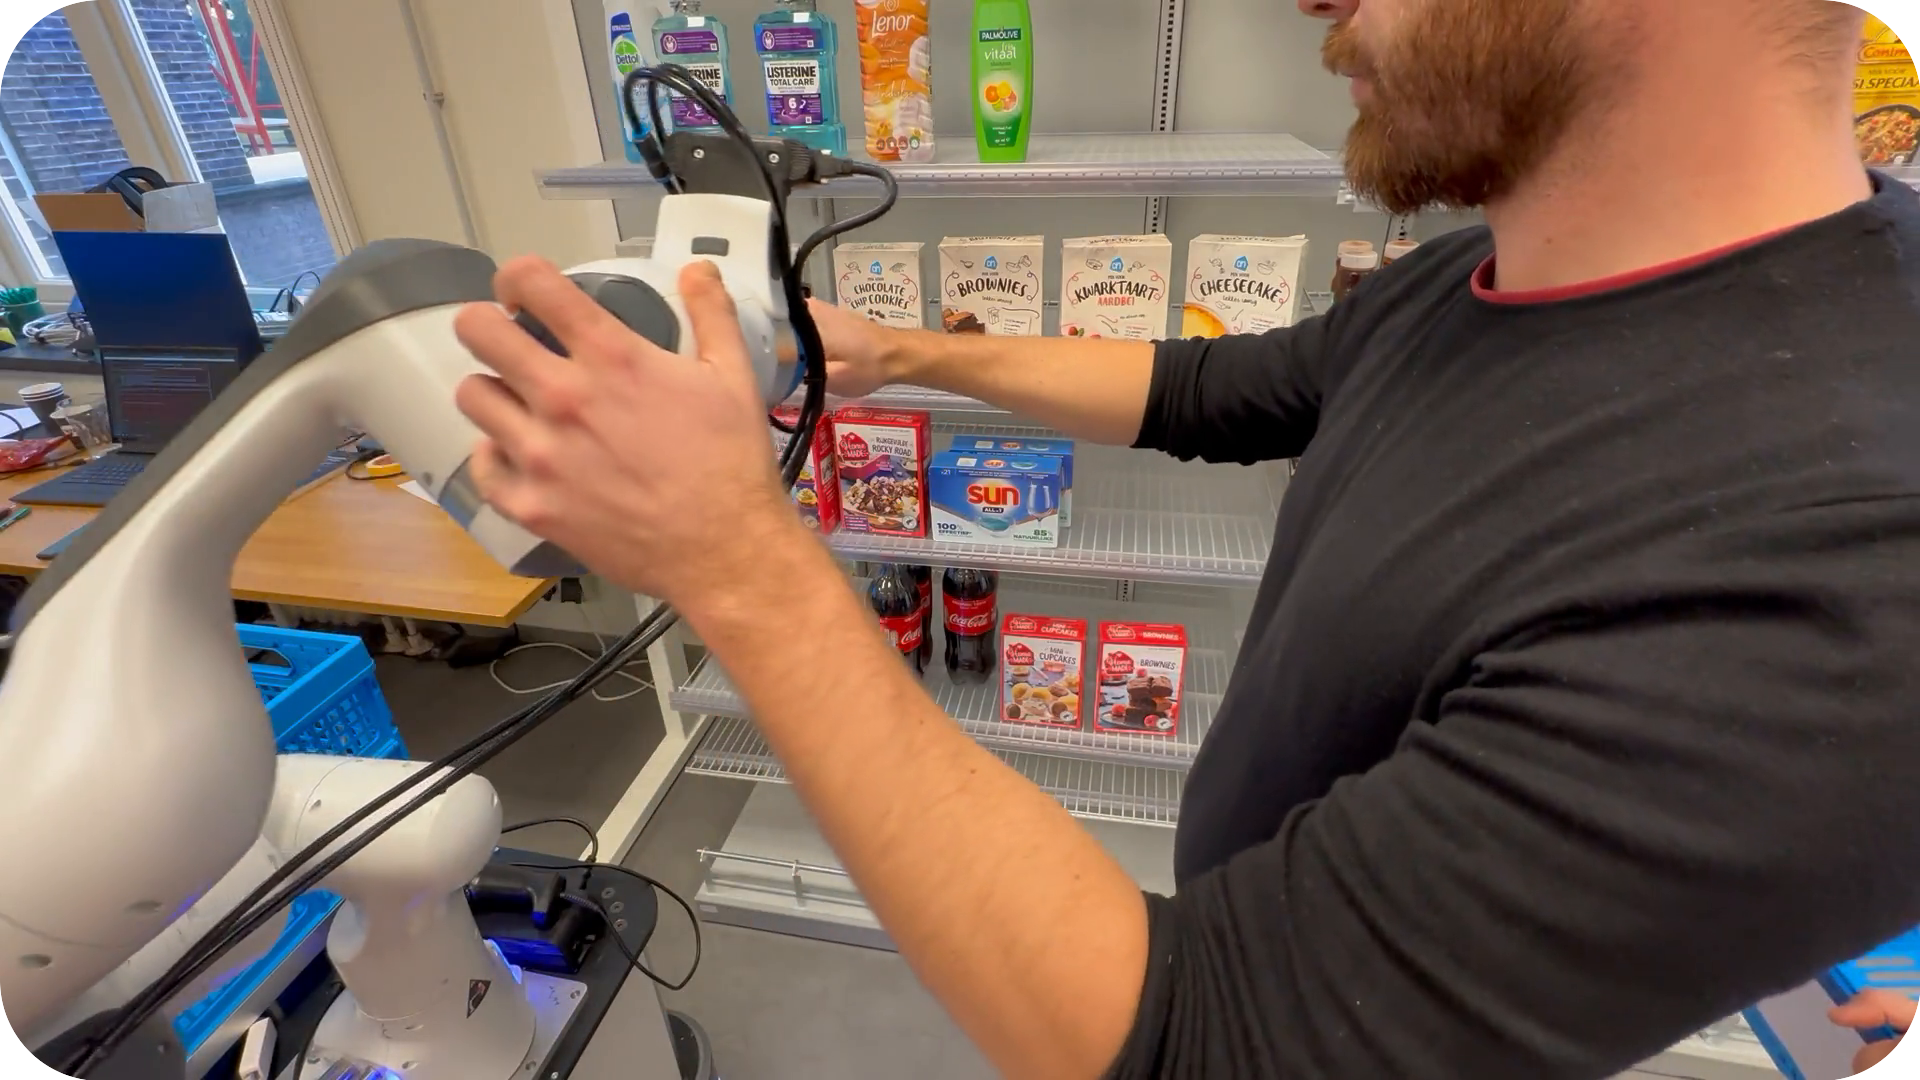
\includegraphics[width=0.95\textwidth]{teaching_005_rounded.png}
    \caption{}
    \label{subfig:teaching_1}
  \end{subfigure}
  \begin{subfigure}[b]{0.45\linewidth}
    \centering
    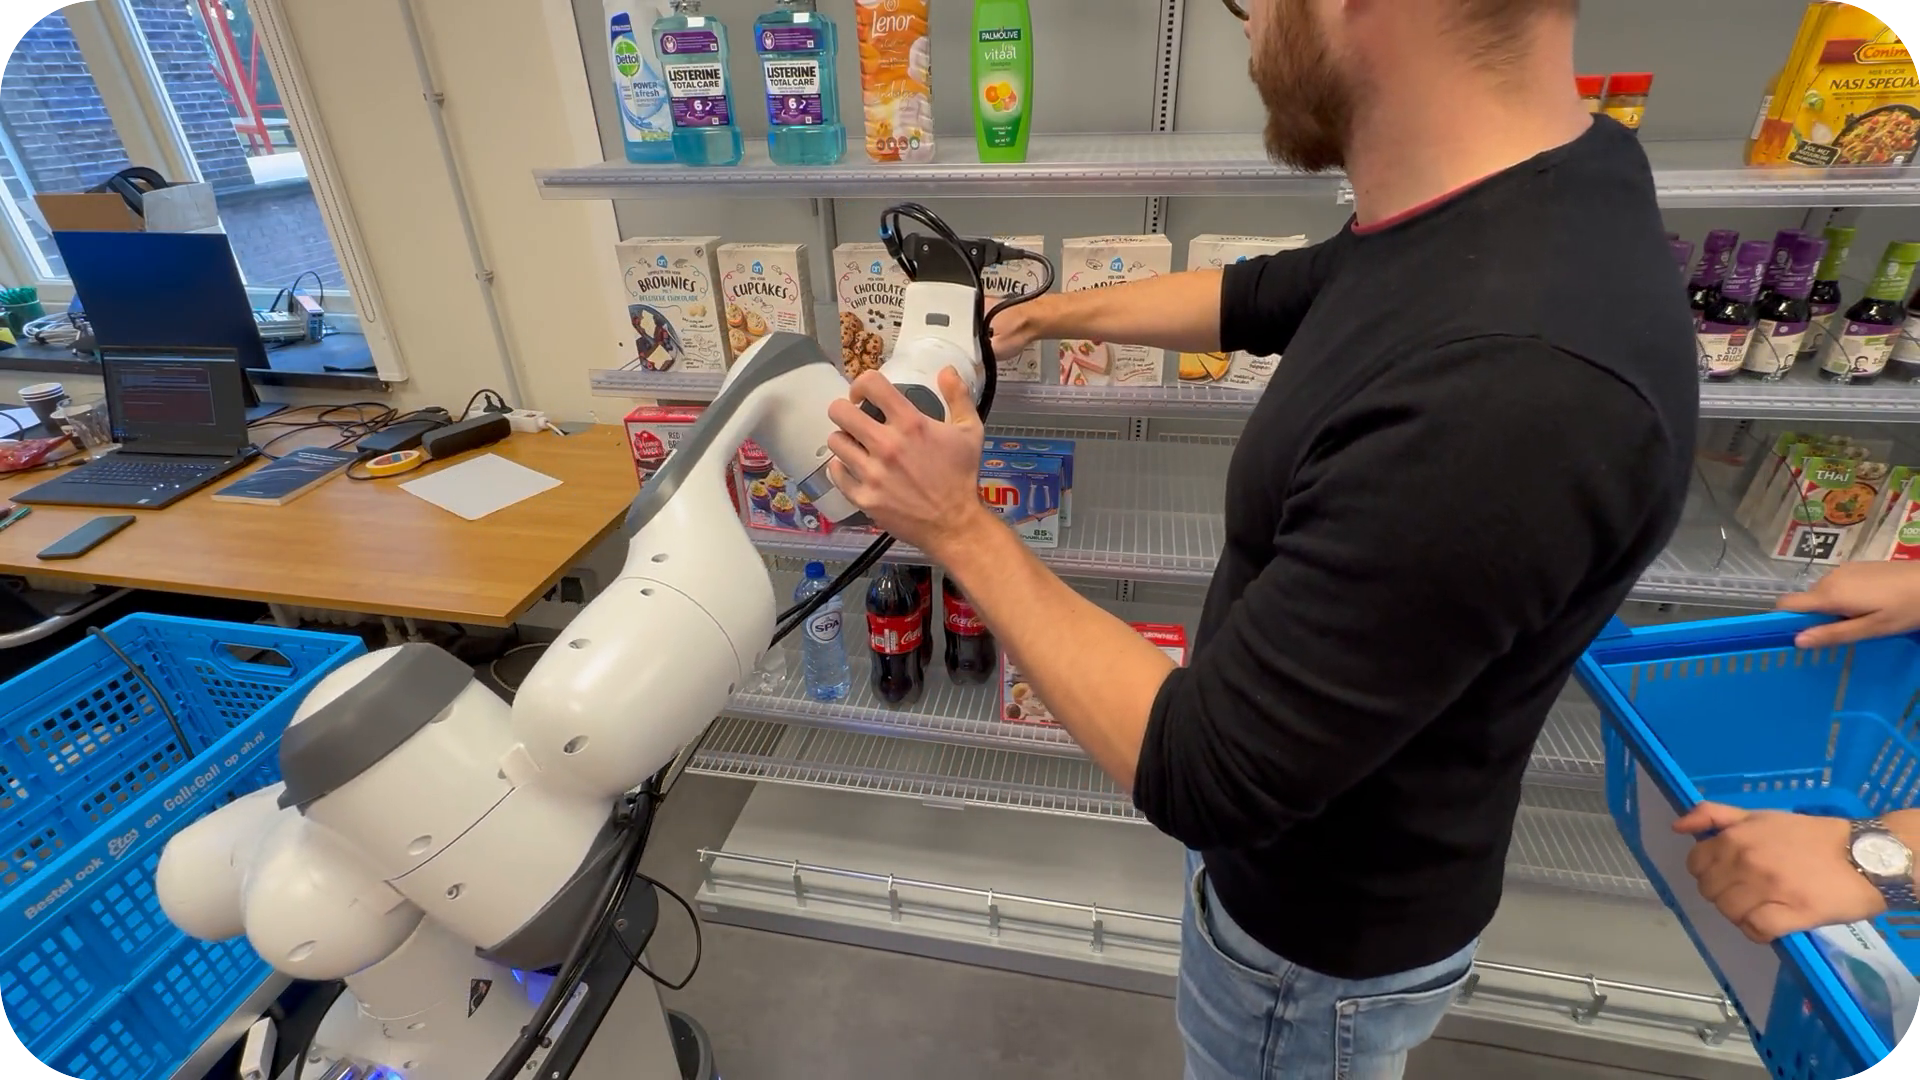
\includegraphics[width=0.95\textwidth]{teaching_009_rounded.png}
    \caption{}
    \label{subfig:teaching_2}
  \end{subfigure}
  \begin{subfigure}[b]{0.45\linewidth}
    \centering
    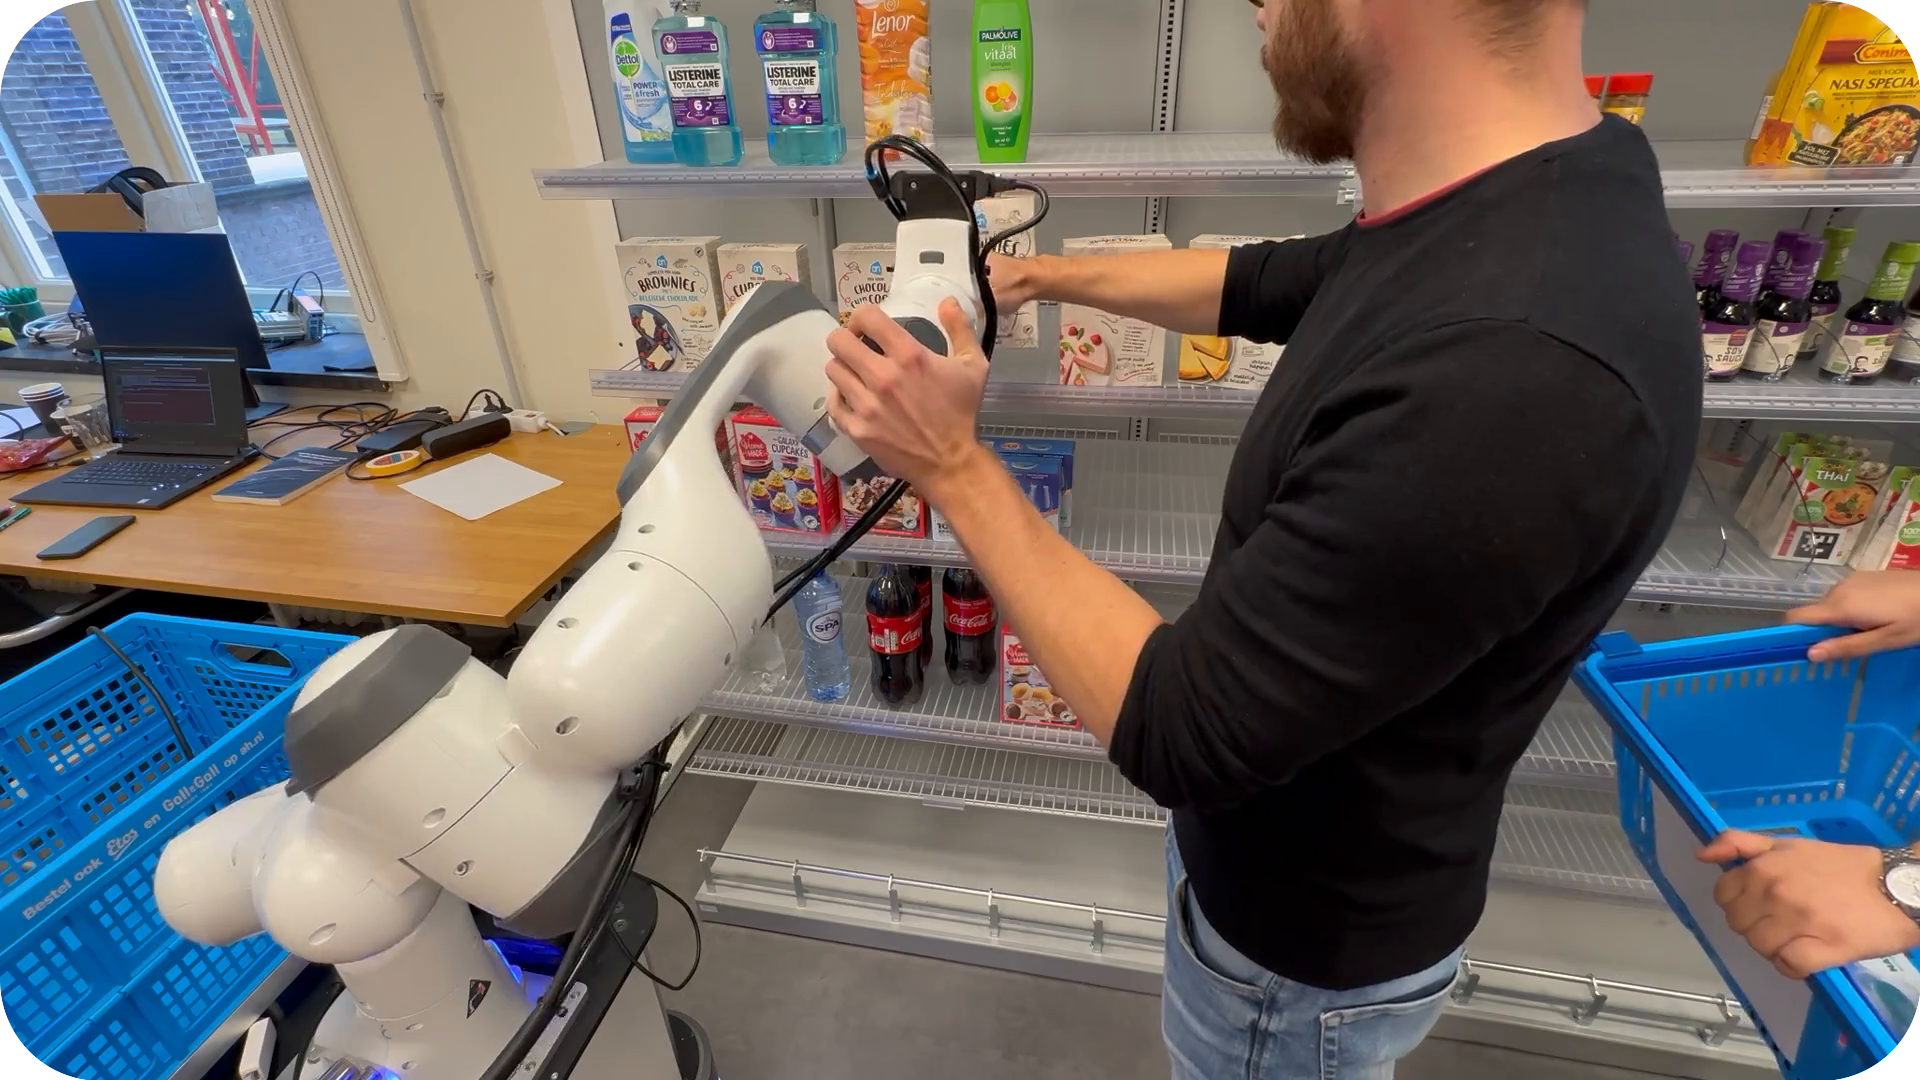
\includegraphics[width=0.95\textwidth]{teaching_011_rounded.png}
    \caption{}
    \label{subfig:teaching_3}
  \end{subfigure}
  \begin{subfigure}[b]{0.45\linewidth}
    \centering
    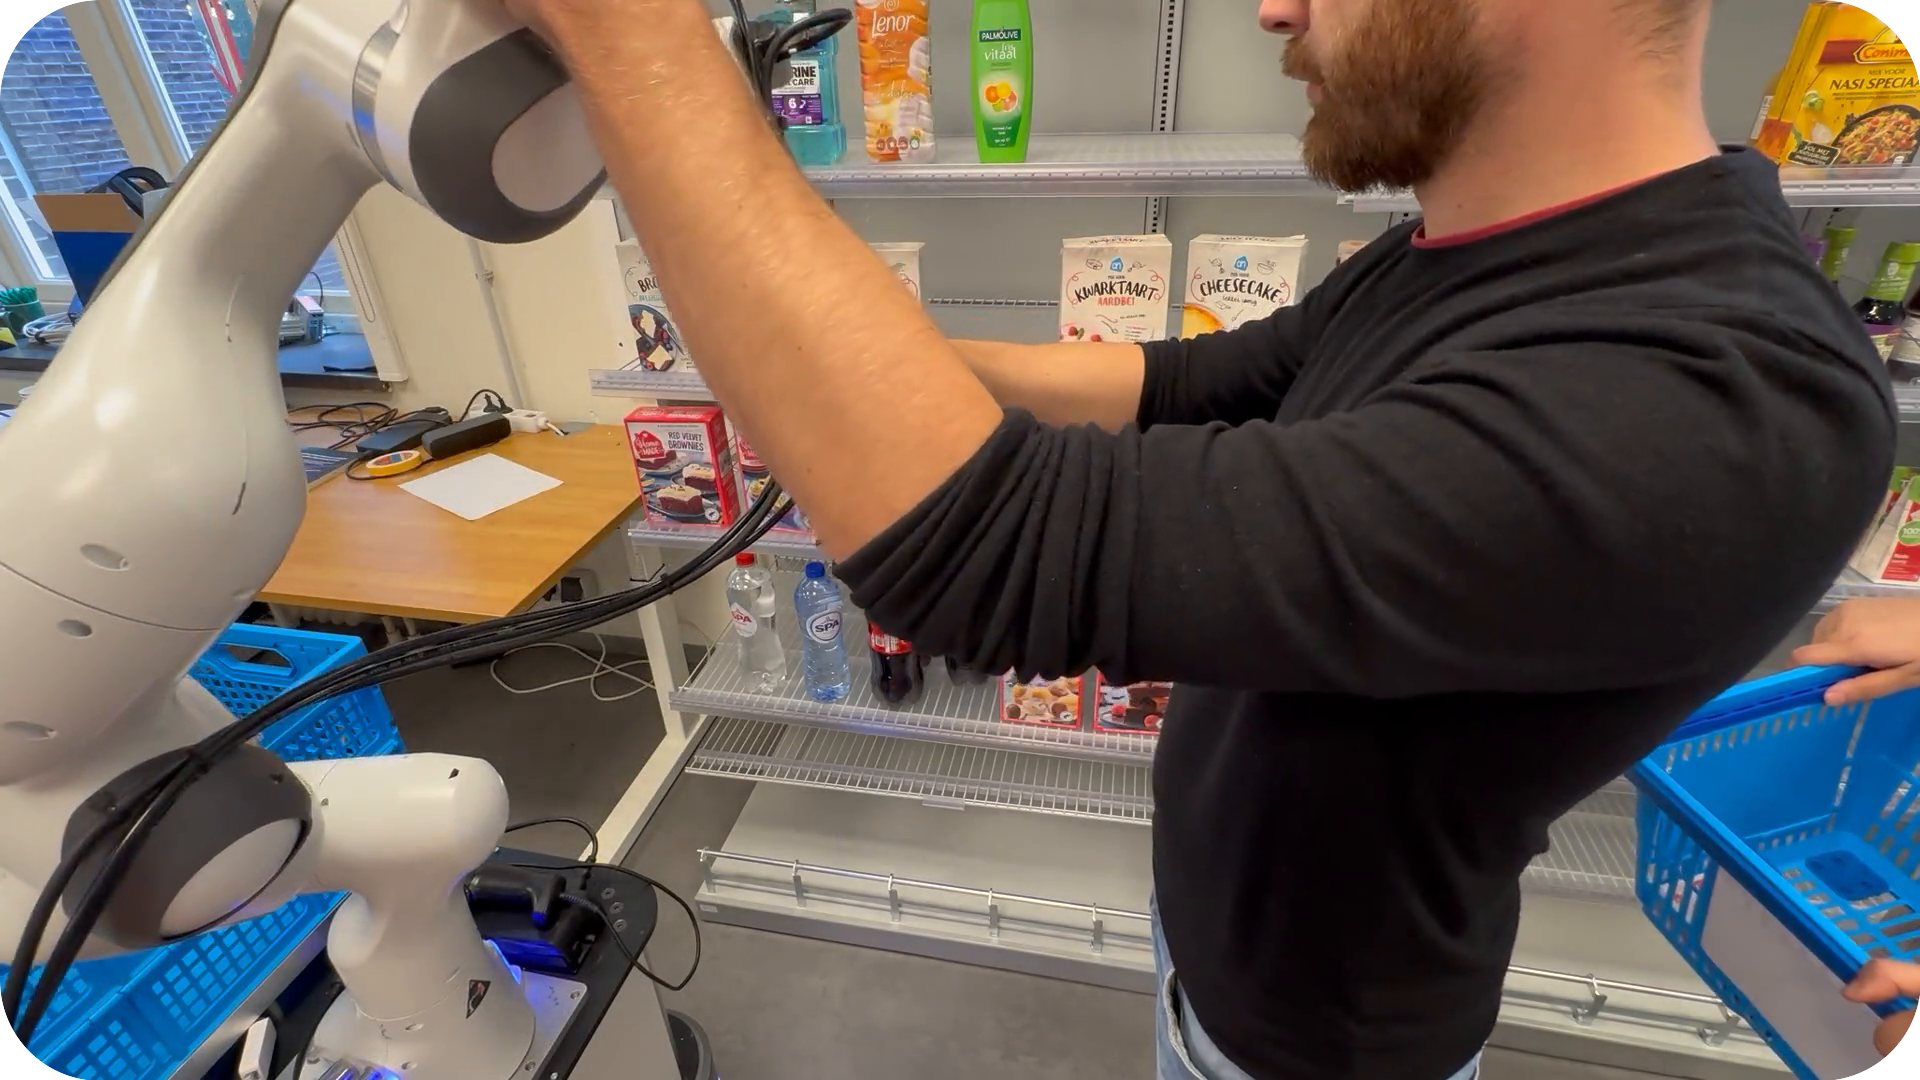
\includegraphics[width=0.95\textwidth]{teaching_014_rounded.png}
    \caption{}
    \label{subfig:teaching_4}
  \end{subfigure}
  \caption{The human operator can easily `teach' the robot a new picking
  strategy by moving the arm, thus passing implicit knowledge to the
  robot.}
  \label{fig:recording}
\end{figure}
\subsection{Interactively adding product classes to perception}
\cref{sec:perception} explains ProtoProductNet, our
adaptation to the state-of-the-art ProtoNet, to make the
few-shot learning approach scalable for the supermarket
environment. To add new unseen product classes to
ProtoProductNet, we developed a custom user interaction for
human operators. The interaction contains the following
steps 1) the operator uses a barcode scanner, attached to
the robot, to scan the new product 2) the operator puts the
product in view in front of the robot's camera 3) a GUI with the view of the camera pops up on the screen and the operator interactively drags a box around the new product. The robot should already start detecting the product, as can be verified by a bounding box appearing on screen. To further enhance the detection the operator can add images from different angles of the product. The cropped images selected by the operator are saved locally and combined with the product's barcode. If the same barcode is encountered in future orders, our perception pipeline will now know how to classify the product accurately, without retraining the network.

\subsection{Teaching grasping trajectories to the robot}
\label{sub:teaching}

As outlined in \cref{sec:trajectory_generation},
\ac{fabrics} require global guidance to effectively execute
complex symbolic actions that are essential for some products, see
\cref{fig:product_examples}.
To simplify the process of obtaining this guidance in the form of trajectories, we leverage human expert demonstrations, effectively teaching the robot.
We distinguish between two
phases for teaching, the \textit{recording} and the
\textit{playback}. For both phases, we assume that the product
is visible and detected by the robot, such that we can
compute a transformation between the root link and the product.

\subsubsection{Recording}
When recording a trajectory, we first reduce the stiffness
of the robot to the bare minimum, such that it can easily be
pushed around by the human operator. Then, the human
operator can activate recording by pressing a button on our tablet interface. From that moment onwards, the state values \x{} for the
constraints defined for picking in \cref{sub:picking}
are recorded, see \cref{fig:recording}.
The state of the gripper, active
or non-active, and whether a product is attached to the gripper
are also recorded.
The generated sequence of constraint values and gripper
states is stored as a reference trajectory.

%For the sake of memory efficiency, we
%ignore trajectory points if they are too similar to the
%previous one.
We additionally record the
transformation matrix between the root link of our kinematic
chain and the product to be picked. That allows us to later
generalize the recording to different product poses by applying a rigid body transformation to the trajectory.


\subsubsection{Playback}

During trajectory playback, we loop through the recorded goals sequentially, continuing when a desired goal accuracy has been reached. 
%When playing back a trajectory, the trajectory points are
%passed to the trajectory generator as goals in a sequential
%manner. Proceeding to the subsequent trajectory point
%requires that the current one has been reached up to a
%desired accuracy. 
\begin{figure}[h]
  \centering
  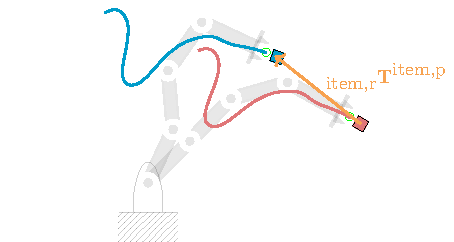
\includegraphics[width=1\linewidth]{trajectory_transformation.pdf}
  \caption{To generalize to different item poses, recorded
  trajectories (red) are transformed based on the the
  transformation between the item's pose during recording
  and during playback (orange). The new trajectory (blue) is then
  tracked using our trajectory generation method.
  }
  \label{fig:transformation_trajectory}
\end{figure}
%
In contrast to the recording part, where we exclude motion
of the base, during playback the base motion is activated,
see \cref{fig:base_motion}. To account for different product
poses between recording and playback, we transform the goals
on the fly based on the product pose estimate, see
\cref{sec:perception}, using the following transform:
\[
  _{\product,r}\mat{T}^{\product,p} =
  \left(_{\textrm{base}}\mat{T}^{\product,r}\right)^{-1}_{\textrm{base}}\mat{T}^{\product,p},
\]
where $_{\textrm{base}}\mat{T}^{\product,r}$ is the transformation matrix
between the manipulator's base link and the product during
recording and $_{\textrm{base}}\mat{T}^{\product,p}$ is the
transformation matrix between the manipulator's base link and
the product during playback, see
\cref{fig:transformation_trajectory}.
Using this continual feedback we effectively employ a visual servoing \cite{kmich2022image} approach and are robust against changes in product location during the pick.
In addition to \ac{fabrics} goals, the recording also contains information about the state of the vacuum pump. This state information is replicated during playback, and used to know when a product should have been attached.
In the playback routine for picking we then modify the fabrics goal if a product is not yet attached where it is expected. The goal is modified to effectively push further into the shelf along the z-axis of the nozzle head, until a product is attached, or a maximum threshold is reached.
\begin{figure*}[t]
  \centering
  \begin{subfigure}[b]{0.20\linewidth}
    \centering
    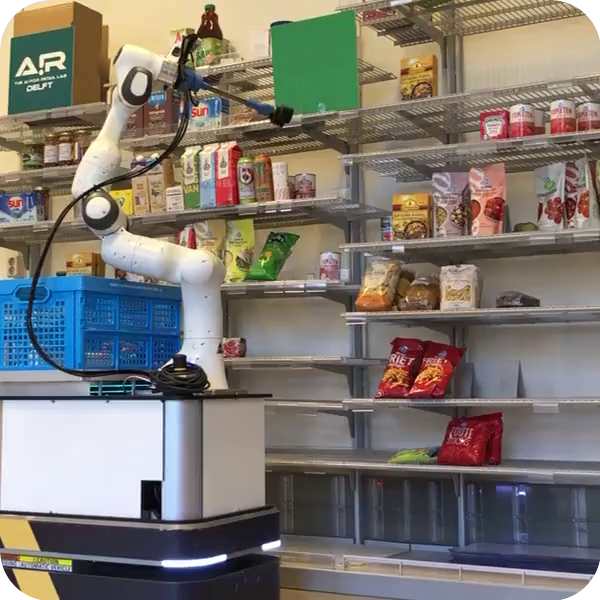
\includegraphics[width=0.95\textwidth]{base_motion_002_rounded_wo.png}
    \caption{}
    \label{subfig:base_motion_1}
  \end{subfigure}
  \begin{subfigure}[b]{0.20\linewidth}
    \centering
    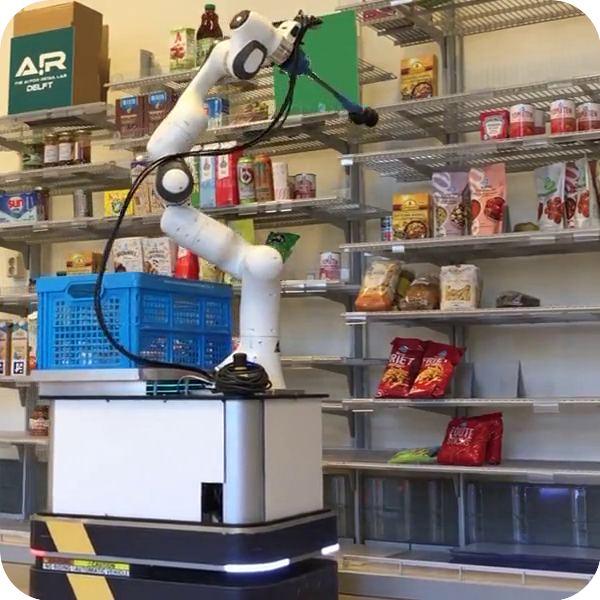
\includegraphics[width=0.95\textwidth]{base_motion_003_rounded_wo.png}
    \caption{}
    \label{subfig:base_motion_2}
  \end{subfigure}
  \begin{subfigure}[b]{0.20\linewidth}
    \centering
    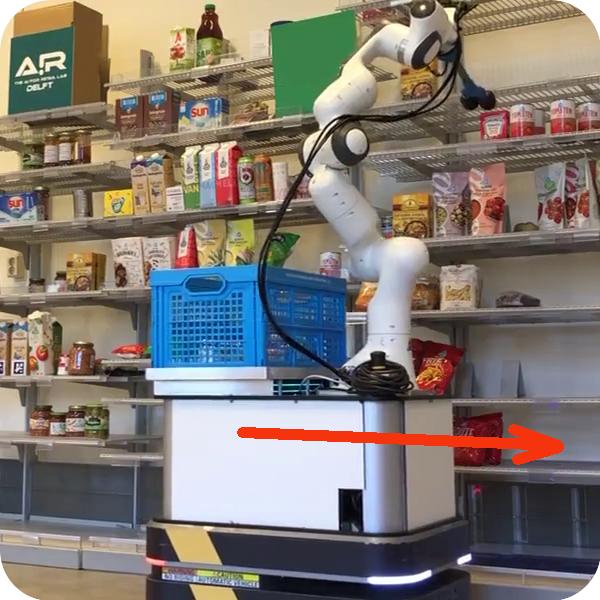
\includegraphics[width=0.95\textwidth]{base_motion_004_rounded_wo.png}
    \caption{}
    \label{subfig:base_motion_3}
  \end{subfigure}
  \begin{subfigure}[b]{0.20\linewidth}
    \centering
    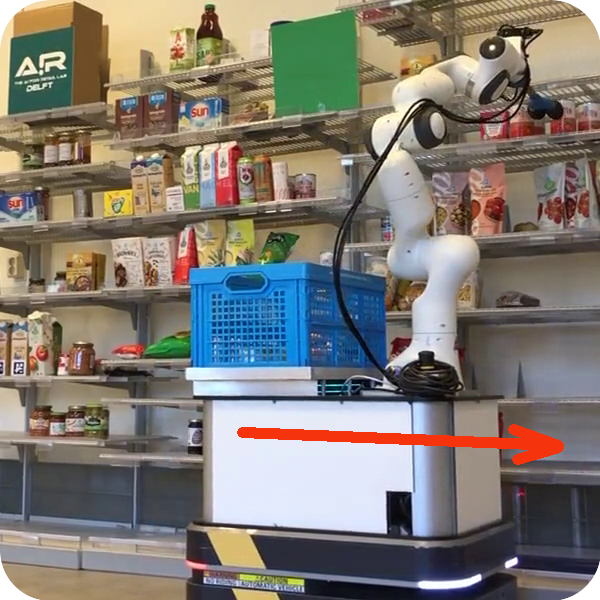
\includegraphics[width=0.95\textwidth]{base_motion_005_rounded_wo.png}
    \caption{}
    \label{subfig:base_motion_4}
  \end{subfigure}
  \caption{During playback, \ac{fabrics}  actively use the base's forward motion as a prismatic joint to compensate for misplacement during navigation.}
  \label{fig:base_motion}
\end{figure*}
%
\subsection{Generalizability}
\label{sub:generalizability}

To reduce the number of taught trajectories, we rely
on generic trajectories. Our gripper design led to 
a \textit{horizontal} and a \textit{vertical} pick
trajectory, where the two suction cups are either aligned
horizontally or vertically. As most considered products have a planar surface, we can use these two
trajectories for most products. These trajectories are
replaced by product specific trajectories in case of
repeated failures. For example, unconventional bottle
shapes require modified trajectories. Similar to existing
works on learning-from-demonstration \cite{argall2009survey}, we
argue that non-experts can, over time, create an increasingly
complete trajectory database for all products to further
improve performance. Importantly, general trajectories have
proven to be sufficient for most of our products.
Note that all trajectories are robot agnostic and only
gripper specific, so we expect them to be transferable to
other robots with similar gripper designs.
The generalizability of our approach relies on the
transformation of trajectories according to the item's pose. The robot's workspace is a natural limitation, as items placed outside the workspace
(i.e. on the lowest or highest shelf or at the back on the
shelf) are kinematically unreachable and thus, not resolvable by our teaching approach.


\subsection{Audio feedback}
\label{sec:language_feedback}

During the robot's operation, we are interested in providing
audio explanations of the robot's actions as feedback to
operators, e.g., to monitor the robot and to be notified
about failures. We do this by 1) generating compact prompts
of the robot's action and state and 2) using Large Language
Models (LLMs) to generate short informative explanations
that are played via the robot's speaker.


\paragraph{Prompt generation}
We leverage the structure of the generated \acp{bt} and
symbolic state information (see \cref{sec:decision_making})
to generate prompts for an LLM. For every sub-tree in the
generated \ac{bt}, we automatically add explanation
nodes that
generate prompts for symbolic actions and items. An
explanation is
described by its name $a$ formulated as a verb in the
present continuous form, e.g., $a=\texttt{placing}$. The
item's name $i$ is taken from the product database, e.g.,
$i=\textit{Whole Milk}$. We generate string prompts of the
form $pr$:
\begin{equation*}
    pr := \textit{action }~a~i~c,
\end{equation*}
where $c\in\{\texttt{running},\texttt{failed}, \texttt{completed}, \texttt{retry}\}$ is the status returned from the sub-tree.
An example for a generated prompt is ``\textit{action }\texttt{picking }\texttt{Whole Milk }\texttt{retry}''.


\paragraph{Explanation generation}
We generate explanations by prompting an LLM on the fly with our generated prompts. 
To this end, we provide the LLM with a context describing
that the robot is deployed as an order picking robot in a
supermarket with five symbolic actions and that the task is to generate a concise explanation of the prompt to operators. 
During operation of the robot, we simultaneously generate the explanations and play them back via the robot's speaker.
For instance, for the prompt  ``\textit{action }\texttt{picking }\texttt{Whole Milk }\texttt{retry}'', we generate the explanation: ``Oops! It seems like I had a little trouble placing the Whole Milk into my basket. No worries, I'll give it another
  try and make sure it goes in smoothly this time''.


\section{Experimential results}
\label{sec:results}

This work does not only proposes three new methods to realize collision
avoidance in dynamic environments with \ac{fabrics}, but it also includes an
analysis of the different methods under noisy sensor data. In the real world, 
sensor data, but also the perception pipeline detecting obstacles and occupied
voxels, produces sensor noise. In this section, we present quantative
comparisons for three simulation environments, namely a holonomic ground robot,
a non\hyp{}holonomic ground robot and a robot manipulator. For all cases, we evaluate
50 cases with different noise levels $\sigma$. The noisy signal is generated
using a Gaussian distrubtion centered around the unoisy sensor data. 
The performance is measured 
in terms of sucess, solver time and execution time to reach the goal. Lastly, 
we evaluate the methods in the real world using a real manipulator.

\begin{figure}
  \begin{subfigure}{0.5\linewidth}
    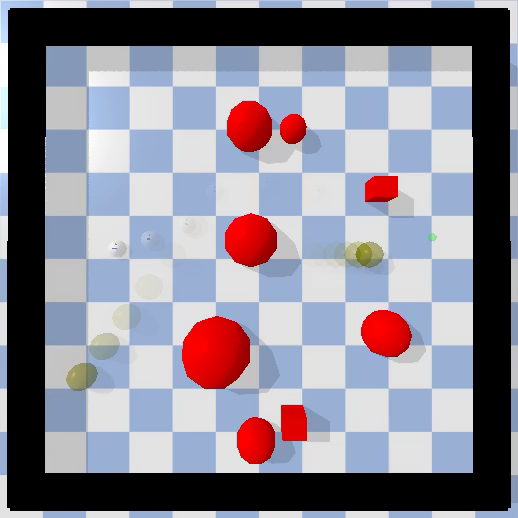
\includegraphics[width=0.95\linewidth]{point_robot_sim/case}
    \caption{Point Robot Case}
    \label{fig:point_robot_case}
  \end{subfigure}%
  \begin{subfigure}{0.5\linewidth}
    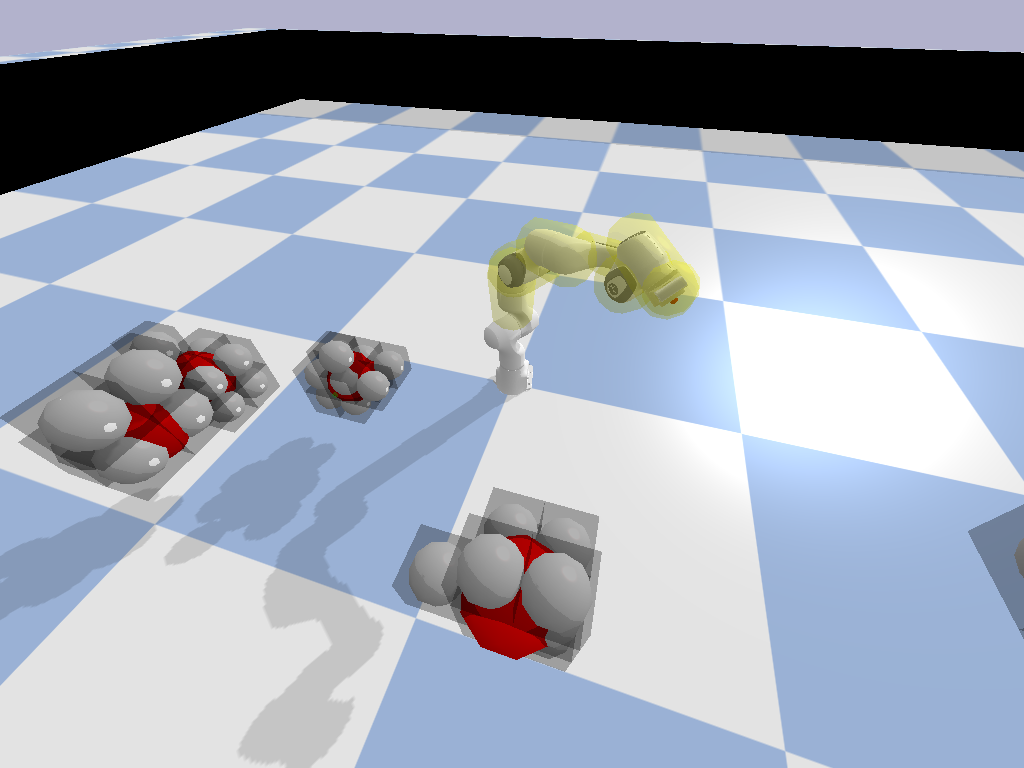
\includegraphics[width=0.95\textwidth]{methods/raw_sensors_panda.png}
    \caption{Occupancy Grid}
    \label{fig:panda_raw_sensors}
  \end{subfigure}%
\end{figure}


\paragraph{Details on implementation}
The planner's implementation can be found at
\href{www.github.com/tud-amr/fabrics}{Geometric Fabrics}. The simulation
environment as well as the the algorithm for computing the \ac{fsd}, \ac{sdf}
and the raw lidar data can be found as part of
\href{www.github.com/maxspahn/gym_envs_urdf}{urdfenvs}. For the real world
experiments, we used a ros bridge and used the same
implementation to process the real point cloud generated by
a highly reactive octomap \cite{Hornung2013}.

\subsection{Point Robot}
\label{sub:point_robot}

When comparing explicit environment representations with the proposed techniques
using noise-free sensor data ($\sigma=0.0$), \acp{sdf} demonstrate the highest
success rate. This is likely due to the \textit{guidance} provided by the
\ac{sdf}'s gradient information. However, intriguingly, the explicit method's
performance appears to improve with increasing noise ($\sigma$), warranting
further investigation.

The goal reaching times remain similar across all approaches, which aligns with
expectations as the tuning is based on this criterion, as shown in
\cref{subfig:point_robot_sim_time2Goal}. While solver computation times are low
for all methods (approximately $3.5$ ms), utilizing raw lidar data substantially
increases computational costs, as observed in
\cref{subfig:point_robot_sim_solvertimes}. This increase results from accounting
for a greater number of obstacles compared to the other methods.


\begin{figure}[ht]
  \centering
  \begin{subfigure}{0.33\linewidth}
    \centering
  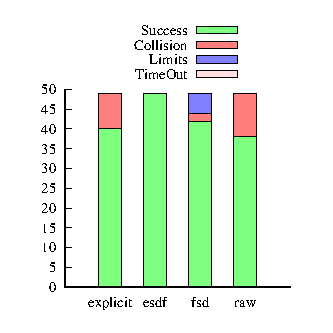
\includegraphics[width=1.0\textwidth]{point_robot_sim/success_PointRobot_00}
    \caption{$\sigma = 0.0$}%
    \label{subfig:point_robot_sim_sucess_noise_00}
  \end{subfigure}%
  \begin{subfigure}{0.33\linewidth}
    \centering
    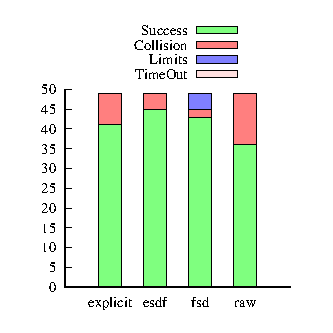
\includegraphics[width=1.0\textwidth]{point_robot_sim/success_PointRobot_01}
    \caption{$\sigma=0.1$}%
    \label{subfig:point_robot_sim_success_noise_01}
  \end{subfigure}%
  \begin{subfigure}{0.33\linewidth}
    \centering
    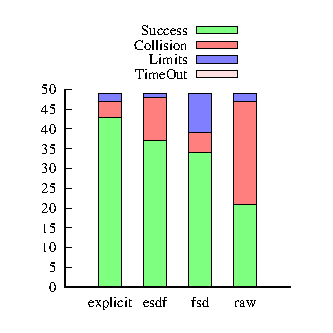
\includegraphics[width=1.0\textwidth]{point_robot_sim/success_PointRobot_02}
    \caption{$\sigma=0.2$}%
    \label{subfig:point_robot_sim_success_noise_02}
  \end{subfigure}%
  \caption{Point robot in simulation.
  }%
  \label{fig:point_robot_sim_success}
\end{figure}

\begin{figure}[ht]
  \centering
  \begin{subfigure}{0.5\linewidth}
    \centering
  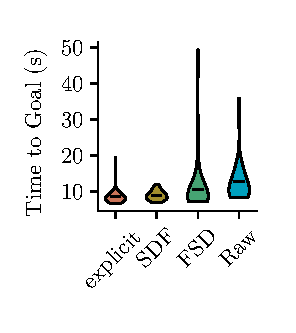
\includegraphics[width=0.9\textwidth]{point_robot_sim/time2Goal_PointRobot_00}
    \caption{Goal reaching time}%
    \label{subfig:point_robot_sim_time2Goal}
  \end{subfigure}%
  \begin{subfigure}{0.5\linewidth}
    \centering
    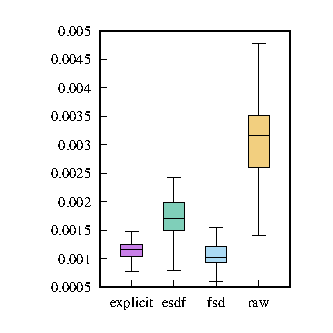
\includegraphics[width=0.9\textwidth]{point_robot_sim/solvertime_PointRobot_00}
    \caption{Solvertimes}%
    \label{subfig:point_robot_sim_solvertimes}
  \end{subfigure}%
  \caption{Point robot in simulation.
  }%
  \label{fig:point_robot_sim_metrics}
\end{figure}

\subsection{Panda}
\label{sub:panda}

When examining results obtained with the \ac{panda} robot, there is a notably
greater variance in performance compared to those observed with the point robot.
Notably, it becomes evident that \ac{fabrics} exhibit heightened robustness in
dynamic environments marked by noisy sensor data, particularly when employing
\ac{fsd}. This approach maintains a high success rate as noise levels escalate,
in contrast to the significant performance degradation observed with other
methodologies, as depicted in \cref{fig:panda_sim_success}.

Furthermore, \ac{fsd} boasts the shortest computational times, approximately $1$
ms. This underpins the conclusion that in dynamic settings, \ac{fsd} harmonizes
most effectively with the \ac{fabrics} framework. This finding aligns with
outcomes from receding horizon optimization techniques, such as those
highlighted in \cite{Tordesillas2019}, applied to \ac{mpc} formulations
involving drones.

\begin{figure}[ht]
  \centering
  \begin{subfigure}{0.33\linewidth}
    \centering
    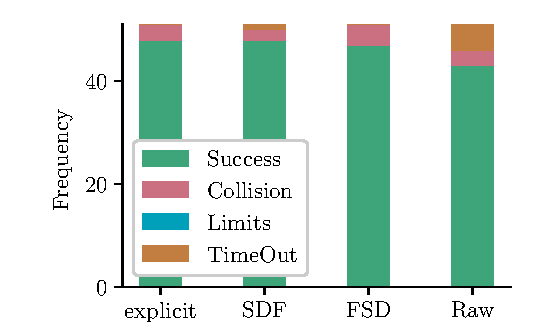
\includegraphics[width=1.0\textwidth]{panda_sim/success_Panda_00.eps}
    \caption{$\sigma = 0.0$}%
    \label{subfig:panda_sim_sucess_noise_00}
  \end{subfigure}%
  \begin{subfigure}{0.33\linewidth}
    \centering
    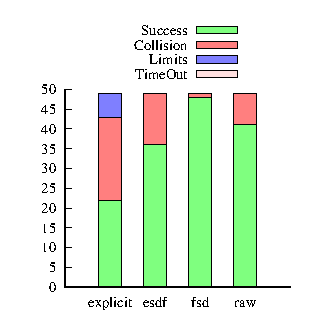
\includegraphics[width=1.0\textwidth]{panda_sim/success_Panda_005.eps}
    \caption{$\sigma=0.05$}%
    \label{subfig:panda_sim_success_noise_005}
  \end{subfigure}%
  \begin{subfigure}{0.33\linewidth}
    \centering
    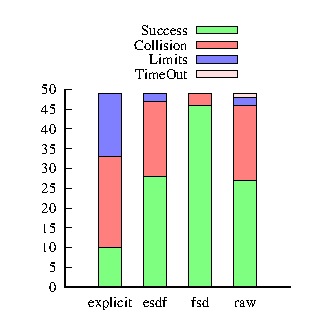
\includegraphics[width=1.0\textwidth]{panda_sim/success_Panda_01.eps}
    \caption{$\sigma=0.1$}%
    \label{subfig:panda_sim_success_noise_01}
  \end{subfigure}%
  \caption{Panda robot in simulation.
  }%
  \label{fig:panda_sim_success}
\end{figure}

\begin{figure}[ht]
  \centering
  \begin{subfigure}{0.5\linewidth}
    \centering
  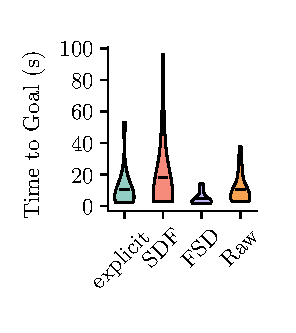
\includegraphics[width=0.9\textwidth]{panda_sim/time2Goal_Panda_00}
    \caption{Goal reaching time}%
    \label{subfig:panad_sim_time2Goal}
  \end{subfigure}%
  \begin{subfigure}{0.5\linewidth}
    \centering
    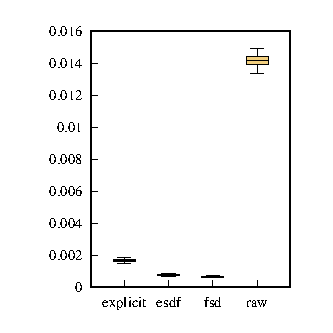
\includegraphics[width=0.9\textwidth]{panda_sim/solvertime_Panda_00}
    \caption{Solvertimes}%
    \label{subfig:panad_sim_solvertimes}
  \end{subfigure}%
  \caption{Panda robot in simulation.
  }%
  \label{fig:panad_sim_metrics}
\end{figure}

\subsection{Real-World Experiments} % (fold)
\label{sub:real_world_experiments}



\section{Lessons Learned and Key Takeaways}

Throughout our project, we have gained valuable insights that inform our approach to deploying robotic systems effectively. These lessons, drawn from hands-on experience, highlight key considerations and strategies we believe essential for successfully implementing robotic software solutions.

\begin{itemize}

    \item \textbf{Human expert trajectories are an efficient way of encoding grasping strategies}: 
    Through the recording of human expert picking
    trajectories, we could address a significant portion of
    collision avoidance challenges and grasping strategies
    for specific products. This approach effectively allows
    for the encoding of per product strategies regarding
    grasp approach, location, and retrieval in a far more
    streamlined manner compared to traditional hard-coded
    behaviors.
    We showed that default trajectories
    generalize for various similarly shaped products, so
    that the number of trajectories can be much lower than
    the number of different products.
    Although the adaptation of recorded
    trajectories proved successful, we require more complex
    methods to mitigate remaining failure cases.
    
    \item \textbf{Accurate product detection and continuous visual feedback are crucial}:
    Accurate product detection and pose estimation emerged as critical requirements within the confines of supermarket environments because of the small size of certain products and the lack of clearance. Continuous visual feedback, particularly through visual servoing techniques, played a pivotal role by enabling real-time tracking of products and refining pose estimations as the robotic arm approached the target object.

    \item \textbf{Vacuum grippers may fail with light and small products}:
    We underestimated the inherent difficulty in effectively picking very light and small products. This challenge highlights the need for alternative gripping mechanisms or specialized approaches tailored to handling such delicate items.

    \item \textbf{Grasping angles heavily influence seal integrity and stability}:
    We put particular emphasis on selecting optimal grasping angles to ensure both seal integrity and product stability during suction grasping. Preferably, the grasp is positioned on a product's flat side  to establish a secure seal while minimizing the risk of product displacement or toppling. A slight angle of approach that gently presses the product against the surface further enhances stability.

    \item \textbf{Compliant robots are key in dynamic environments}:
    Compliance is essential when safely operating rigid robotic arms in dynamic environments and alongside humans.
    To guarantee collision avoidance with humans requires
    accurate human detection and intent detection. As this
    is highly complex, we opted for safety through
    compliance during arm motion and rely on raw lidar data
    during base motion.
    Beyond safety, compliance offers inherent forgiveness in the event of grasping failures. Together with our adaptive online task planner, this combination enables our robot to recover or retry autonomously, minimizing human interventions. 

    \item \textbf{Whole body control enhances efficiency}:
    Whole body (or semi-whole body) control simplifies the task of picking products from diverse shelves within a supermarket setting. The expanded configuration space with the additional degrees of freedom significantly enhances planning efficiency and reliability, thereby streamlining operations.

    \item \textbf{Rapid and iterative software development is imperative}:
    Rapidly iterating our software directly on the physical robot was a critical success factor for us. Swift iterations serve as a reliable indicator of the eventual outcome. Furthermore, our realistic rest lab environment with anticipated operational conditions enhanced overall system robustness.

    \item \textbf{Lack of high quality mobile manipulators hinders progress}:
    Contrary to prevailing notions, the development of mobile manipulators present substantial challenges, particularly in research. Existing solutions remain scarce, and researchers are often forced to deal with inaccurate and unreliable mobile bases and robotic arms with short battery lives. Similarly, versatile gripper design is an unsolved research topic. This underscores the need for continued exploration and innovation in this domain to bridge existing gaps and facilitate rapid advancements in robotic research.   
\end{itemize}

\section{Conclusion}
\label{sec:conclusion}

This paper introduces several approaches to surpass explicit environment
representations, employing three distinct implicit representations within the
\ac{fabrics} framework. The study demonstrates that these techniques notably
reduce demands and constraints on perception pipelines, while maintaining a low
computational load on the planner. Consequently, the proposed methods enable the
application of analogous strategies in both dynamic and static environments.
The outcomes underline the successful integration of numerical gradients,
frequently accessible in trained models, into the symbolic implementation of
\ac{fabrics} detailed in \cite{Spahn2022}. Future endeavors should concentrate
on incorporating more implicit robot representations as outlined in
\cite{Liu2022regularized,Koptev2023neural} into this framework. While this work refrains from
delving into dynamic environmental dynamics, an exploration of the potential
synergies between the implicit representations introduced here and the findings
from \cite{Spahn2022} is a promising avenue for investigation.


\newpage
